\documentclass[a4paper,10pt,titlepage]{report}
%%This template is based on Paco van Beckhoven's thesis. 

\usepackage{xspace}
\usepackage{xargs}   % Use more than one optional parameter in a new commands
\usepackage[pdftex,dvipsnames]{xcolor}

% Putting images next to each other
\usepackage[font=bf,]{caption}
\usepackage{subcaption}
\input{glyphtounicode}

% for last page
\usepackage{lastpage}

\usepackage[english]{babel}
\usepackage[utf8]{inputenc}
\usepackage{csquotes}
\usepackage[margin=1in]{geometry}
\usepackage{fancyhdr}
\usepackage{booktabs}
\usepackage{paralist}
\usepackage{graphicx}
\usepackage{tabularx}
\usepackage{adjustbox}
\usepackage{titlepic}
\usepackage{vhistory}
\usepackage{enumitem}
\usepackage{longtable}
\usepackage[backend=biber, style=ieee,citestyle=numeric-comp]{biblatex}
\usepackage[colorinlistoftodos, prependcaption]{todonotes}
\usepackage{placeins}
\usepackage{multirow}
\usepackage{amsmath,amssymb}
\usepackage[hidelinks]{hyperref}
\usepackage[acronym,nogroupskip,nohypertypes={acronym},toc,section=chapter]{glossaries}
\usepackage{amssymb}
\usepackage{verbatim}
\usepackage{cmap}
%my additions
\usepackage{url}

%\usepackage[ansinew]{inputenc}
%\usepackage[T1]{fontenc}
%\usepackage{libertine}
\input{glyphtounicode}

\pdfglyphtounicode{f_f}{FB00}
\pdfglyphtounicode{f_f_i}{FB03}
\pdfglyphtounicode{f_f_l}{FB04}
\pdfglyphtounicode{f_i}{FB01}

\pdfgentounicode=1



%Appendix package + appendix in chapter title
\usepackage[titletoc]{appendix}




%for highlighting findings
\usepackage{tcolorbox}

% for highlighting code examples
\usepackage{listings}

\newcommand{\ie}{\emph{i.e.},\xspace}
\newcommand{\eg}{\emph{e.g.},\xspace}
\newcommand{\etc}{\emph{etc.}\xspace}
\newcommand{\etal}{\emph{et al.}\xspace}

\newcommand{\sig}{\gls{sig}}
\newcommand{\sigs}{\glspl{sig}}

\newcommandx{\unsure}[2][1=]{\todo[linecolor=red,backgroundcolor=red!25,bordercolor=red,#1, inline]{#2}}
\newcommandx{\discussion}[2][1=]{\todo[linecolor=red,backgroundcolor=green!25,bordercolor=red,inline,#1]{#2}}

\newcommandx{\improvement}[2][1=]{\todo[linecolor=blue,backgroundcolor=blue!25,bordercolor=blue,#1]{#2}}

\newcommandx{\reminder}[2][1=]{\todo[linecolor=yellow,backgroundcolor=yellow!25,bordercolor=yellow,#1]{#2}}

\newcommandx{\lessprio}[2][1=]{\todo[linecolor=Plum,backgroundcolor=Plum!25,bordercolor=Plum,#1]{#2}}
\newcommandx{\todocontent}[2][1=]{\todo[author=\textbf{Planned content},backgroundcolor=Goldenrod!25,bordercolor=Goldenrod,inline,#1]{#2}}


%%Some additional table column specifiers, allowing for fixed width columns that wrap.
\newcolumntype{L}[1]{>{\raggedright\let\newline\\\arraybackslash\hspace{0pt}}p{#1}}
\newcolumntype{C}[1]{>{\centering\let\newline\\\arraybackslash\hspace{0pt}}p{#1}}
\newcolumntype{R}[1]{>{\raggedleft\let\newline\\\arraybackslash\hspace{0pt}}p{#1}}

\definecolor{ryel}{HTML}{fcd116}
\definecolor{rred}{HTML}{ce1126}
\definecolor{rblu}{HTML}{0a3eb9}
%these are examples of commands that may facilitate feedback annotations in the document
%replace \paco by your name and \ana by your supervisor's name
%\newcommandx{\ana}[2][1=]{\todo[linecolor=rblu,backgroundcolor=ryel,bordercolor=rred,#1]{#2}}
%\newcommandx{\paco}[2][1=]{\todo[author=Paco,linecolor=blue,backgroundcolor=white,bordercolor=red,#1]{#2}}


% -- title page is a modified version of https://github.com/software-engineering-amsterdam/latex/blob/master/thesis/uvamscse.cls
\newcommand{\email}[1]{\ttfamily\href{mailto:#1}{#1}}

\newcommand{\uvacoverfoot}{%
	\vfill
	\begin{center}
		\begin{tabular}{r|l}
			\multirow{3}{*}{
\includegraphics[height=48pt]{uva.pdf}}
			&\textsc{\Large Universiteit van Amsterdam}\\
			&\textsc{Faculteit der Natuurwetenschappen, Wiskunde en Informatica}\\
			&\textsc{Master Software Engineering}\\
			&\url{http://www.software-engineering-amsterdam.nl}
		\end{tabular}
	\end{center}
}

\renewcommand{\maketitle}{%
	% The cover page
	% --------------
	\thispagestyle{empty}
	\enlargethispage{30pt}
	\renewcommand{\thefootnote}{\fnsymbol{footnote}}
	% Will be page 0, s.t. contents start on page 1
	\setcounter{page}{0}
	% \eccoverhead
	% Volume and article title, author(s)
	\vspace{60pt}
	\begin{center}
		{\Huge\bfseries The comparison of the energy consumption of different programming languages and programs \par}
		% Earlier versions:
		% Assessing Test Suite Effectiveness Using Static Analysis
		% Predicting Test Suite Effectiveness Using Static Analysis 
		% Predicting Test Suite Effectiveness Using Static Source Code Analysis 
		% Assessing Test Suite Effectiveness Using Static Analysis
		% Predicting test suite effectiveness using static analysis
		\vspace{44pt}
		{\Large\bfseries Lukas Koedijk \par}
		\email{lukaskoedijk@gmail.com}\\
		\vspace{11pt}
		\today, \pageref{LastPage} pages
	\end{center}
	\vfill
	\begin{tabular}{ll}
		\textbf{Research supervisor:} 	& A. M. Oprescu, \email{a.m.oprescu@uva.nl} \\
		\textbf{Host/Daily supervisor:} & D. Stam, \email{stam.dennis@kpmg.nl}\\
		\textbf{Host organisation/Research group:} & KPMG Advisory N.V., \url{www.kpmg.nl}
	\end{tabular}
	\uvacoverfoot
	\newpage
	\setcounter{footnote}{0}
	\renewcommand{\thefootnote}{\arabic{footnote}}
	\setlength{\parskip}{0pt}
}

%\newcommand{\uvaabstract}{}latex 
%\renewcommand{\abstract}[2][Abstract]{\renewcommand{\uvaabstract}{\chapter*{Abstract}%
%\par#2\newpage}}


%-------- End of ``title page''

%Fancy page headers
\pagestyle{fancy}
\fancyhf{}
\fancyhead[L]{\leftmark}
\fancyfoot[C]{\thepage}
\setlength{\headheight}{14pt}


%%FINDING ENV
\newcounter{findingctr}

\newenvironment{finding}{%      define a custom environment
	\refstepcounter{findingctr}% increment the environment's counter
	\begin{tcolorbox}
	\textbf{Finding \thefindingctr:}
}{\end{tcolorbox}} 
% If you want numbers that start with the chapter or section number (e.g. 7.1.1 or 7.1) enable the following lines 
%\usepackage{amsmath}
%\numberwithin{findingctr}{chapter}


% Decrease the size of all these lists
\setlist{noitemsep,topsep=4pt,parsep=1pt,partopsep=4pt}


\lstset{
	basicstyle=\footnotesize,        % the size of the fonts that are used for the code
	breakatwhitespace=false,         % sets if automatic breaks should only happen at whitespace
	breaklines=true,                 % sets automatic line breaking
	captionpos=b,                    % sets the caption-position to bottom
	frame=single,                    % adds a frame around the code
	language=Java,                 % the language of the code
	keywordstyle=\bf,
	tabsize=2                       % sets default tabsize to 2 spaces
}

%make it fit more nicely
\setlength\extrarowheight{2pt}


%helpful acronym examples
\newacronym{cc}{CC}{Cyclomatic Complexity}

\newacronym{sut}{SUT}{System Under Test}

\newacronym{strew}{STREW}{Software Testing and Reliability Early Warning}

\newacronym{sig}{SIG}{Software Improvement Group}

\newacronym{sat}{SAT}{Software Analysis Toolkit}

\newacronym{tloc}{TLOC}{Lines Of Test Code}
\newacronym{loc}{LOC}{Lines of Code}

\newacronym{taime}{TAIME}{Test Suite Assessment and Improvement Method}

\newacronym{tqm}{TQM}{Test Quality Model}

\newacronym{tdd}{TDD}{Test-Driven Development}

\newacronym{cor}{COR}{Conditional Operator Replacement}
\newacronym{ror}{ROR}{Relational Operator Replacement}
\newacronym{ast}{AST}{Abstract Syntax Tree}
\makeglossaries
\bibliography{main}

\begin{document}



\maketitle
\chapter*{Abstract}
Here goes your abstract. Be concise, introduce context, problem, known approaches, your solution, your findings.
\tableofcontents
\chapter{Introduction}
\label{ch:introduction}
% Context: what is the bigger scope of the problem you are trying to solve? Try to connect to societal/economical challenges.
% Problem Analysis: Here you present your analysis of the problem situation that your research will address.
% How does this problem manifest itself at your host organisation?
% Also summarises existing scientific insight into the problem.
%maybe not only milieu but also money
Currently more and more people are concerned with global warming. Global warming is partly the result of the emission of greenhouse gasses during energy generation of not green energy options. Because of this a lot of people want to change to green energy generation to help solve this problem. Another solution is to decrease the energy consumption. Which is not only good for the environment but can also save a lot of money on the energy bill. The energy consumption of communication networks, personal computers and data centers world wide is increasing over the years \cite{van2014trends}. This happens with a growth rate of $10\%$, $5\%$ and $4\%$ respectively \cite{van2014trends}. Therefore it is important to research ways of decreasing the energy consumption. In the field of hardware there is, according to Koomey's law, an increase of the number of computations per Joule. However this is not enough, because tasks need more computations to complete due to the confidence in the improvement of hardware \cite{verdecchia2017estimating}. For this reason we need to look at possibilities in decreasing the energy consumption from a software perspective.


\section{Problem statement}
The energy consumption of communication networks, personal computers and data centers are increasing yearly. There are two ways of decreasing the energy consumption, by decreasing the energy consumption of hardware or software. Scientific research is mostly focused on decreasing the energy consumption of hardware. There are also some papers about reducing the energy consumption in the software process and the decision making process. A small bit of research is done on the energy consumption of software, but their research goal is to estimate the energy consumption. Therefore what we miss and are going to look into is if there is a good way of writing code regards the energy consumption.

\subsection{Research questions}
%To tackle these issues, we investigate ...
During this research we answer the following two existence questions: (1) \textbf{Is there a difference in the energy consumption of software projects in different programming languages that have the same functionality} and (2) \textbf{Is there a difference in energy consumption of different software projects (in the same programming language) that have the same functionality}? To answer these questions we first need to answer the three description and classification questions listed below.
\begin{itemize}
    \item How can the energy consumption of a software project be measured?
    \item How do we proof if two programs have the same functionality?
    \item When is a difference in energy consumption big enough to be called a difference?\\
\end{itemize}

Based on the results we find when answering the second existence question, we want to look into what this difference is on code level. To do this we need to answer the descriptive/comparative question \textbf{what is the difference on code level between software project that are in the same programming language and have the same functionality, but have a difference in the energy consumption}? This question is only useful when there is a difference in the energy consumption of software projects in the same programming language that have the same functionality. \\
%Otherwise we can't link the difference in energy consumption to the difference in the code.\\

For the first research question the hypothesis is that there is a difference in the energy consumption based on the programming language chosen. The hypothesis of the second research question is that there is a difference in the energy consumption of different software projects (in the same programming language) that have the same functionality.

\subsection{Research method}
As method we use a controlled experiment. In this experiment we will run different software projects to measure the energy consumption. Here the projects are the variable input, the energy consumption the output and everything else like compiler and energy consumption calculations should be constant.

\subsubsection{Data}
For the first research question we need programs that have the same functionality, but are written in a different programming language. Possible resources for such programs are library code, interview code, student assignments and code from competitions solving math problems. We first looked at library code, but found that libraries most of the time don't use the same algorithm. This is a problem because we don't want to compare algorithms, but the way a programmer writes code. Therefor we used the \textit{the computer language benchmark game} \cite{gouy:2019} as a source for programs that have the same functionality and use the same algorithm for solving the different problems. For the second research question we need programs that have the same functionality and are written in the same language. Here we could also use \textit{the computer language benchmark game} as for most languages there are multiple programs listed.

When proving that all the projects have the same functionality we could have defined properties for the input and output and test if these properties hold for all the projects \cite{mens2004survey}, but \textit{the computer language benchmark game} already makes sure that the programs have the same functionality. Thus we don't have to do this ourselves.

To proof that the projects have different values for the energy consumption we use the one sided Mann Whitney U test. This test has as its hypothesis that two distributions are from the same population.

\subsubsection{Measuring energy consumption}
When measuring the energy consumption of a project you have to take into account the energy consumption of CPU, memory and disk \cite{acar2016impact}. The measurements can be done with a hardware or software approach. A hardware approach is more accurate but also more expensive \cite{acar2016impact}. We want to use a hardware approach and luckily as a student of the UvA we have access to the DAS-4 and the DAS-5. The DAS is a distributed system that can also do energy measurements \cite{bal2016medium}. The nodes that can measure the energy are located at the VU cluster. To measure the energy we need to run a job on the DAS-5 and use the DAS-4 to measure the energy consumption. When running a job we need to specify witch node we want to run the job on, because not all nodes can be measured for the energy consumption. 
%This is done by using the \textit{-w} flag while using the command \textit{srun}. The measuring can then be done by using the \textit{smnpwalk} command and then filtering out the information by using \textit{fgrep Energy}.

\subsubsection{Code level}
When there is a difference in the energy consumption of different software projects in the same programming language we will look at the different projects on code-level. Here we will try to find what is causing a project to have a lower or higher energy consumption. There are too many program combinations to look at, thus we need to make a selection. We choose to look at the languages that had the biggest range in energy consumption for all the problem, these languages are Python, Ruby and PHP. Then we can look for every problem to the two programs that differ the most for those three programming languages. We will look at the program combinations side by side and write down the differences that we see. Then we look at these differences and see if some are occurring more often then others. These findings will then be tested by writing our own two versions, where before testing we think one is written badly regards the energy consumption and one that is written good. We then run the two version and check if the good version has indeed a lower energy consumption using the Mann Whitney U test.

\section{Contributions}
Our research makes the following contributions:
\begin{enumerate}
	\item An energy consumption measurement set-up
	\item A data set of software programs with the same functionality
	\item Comparison of languages energy consumption
	\item Rules for writing good software regards the energy consumption
\end{enumerate}

\section{Outline}
In Chapter~\ref{ch:background} we describe the background of this thesis. 
Chapter~\ref{ch:research} describes ... 
Results are shown in Chapter~\ref{ch:results} and discussed in Chapter~\ref{ch:discussion}. Chapter~\ref{ch:related_work}, contains the work related to this thesis.
Finally, we present our concluding remarks in Chapter~\ref{ch:conclusion} together with future work.


\chapter{Background}
\label{ch:background}
This chapter will present the necessary background information for this thesis. First, we define some basic terminology that will be used throughout this thesis. Next, ...



%compiler
%miss framewrok benchmark game
%energy uitleggen
%miss units uitleggen
%basic statistics: null hypothese, alpha, p, rejecting h0 more valuable
\chapter{Energy measurement}
\label{ch:energy_measurement}
In this chapter we discus the approach used around the energy measurement. We first look into the possibilities that are available to use. After that we will look at options and issues the energy measurement approach has. Finally we show an overview of the set-up used to measure the energy consumption.\\

% Depending on your subject, you might need multiple research chapters. Moreover, depending on how the research questions are linked, you may need to answer them one by one and then connect the answers into a final discussion chapter. 

% See Canvas for examples of theses with various approaches to structuring the research content.

%energy of system or program
When doing energy measurements it is important to not only measure the energy consumption of the CPU, but also of the memory and disk \cite{acar2016impact}. You can use a hardware method to measure the energy consumption or use a software method to estimate the energy consumption. Using a hardware method is more accurate, but also more expensive \cite{acar2016impact}. This research uses a hardware approach and utilizes the DAS-4 and DAS-5 systems. \\
%The DAS is a distributed supercomputer with nodes that have different hardware specifications and some nodes are connected to a Power Distribution Unit (PDU), through which we can measure the energy consumption \cite{bal2016medium}. This PDU is from Racktivity and has an error marge of 1\%.\\

%The DAS has a head node where all the users connect to. Here the users can reserve nodes and add jobs to the queue. There are multiple releases of the DAS, currently only DAS-4 and DAS-5 are in use. For measuring the energy consumption we needed to run the programs on a specific set of six nodes on the DAS-5. To retrieve the data from the PDU connected to these six nodes we needed to use the DAS-4 and make a connection to the PDU with the use of the Simple Network Management Protocol (SNMP). 
There were two kind of energy measurement values we could retrieve from the PDU, the current power (Watt) and the energy consumption (kWh) from when the node was plugged-in till the moment this value is retrieved. Both methods have a disadvantage when applied. When using the current power one needs to retrieve the power constantly and some accuracy is lost because we don't know what happens with the power draw in between two measure points. The method of measuring the energy consumption has the problem of showing a number that is too large, the numbers are in kWh with a low precision. Thus the lowest decimal shows Watt per hour. We found that for small programs it is not sufficient to only measure in Watt per hour, because of the short run times. We tested this with three programs, an idle program where the only command was \textit{sleep} and two programs that calculates the 10.000th prime one recursively and optimized. The results of this test are shown in figure \ref{tab:EMmethod}. Here we see that the difference of 0.001 kWh is a large difference when working with numbers that are of scale 0.005 kWh. There isn't a clear difference between primes optimized and the sleep that takes close to the same amount of seconds as the primes optimized. Because of these results we choose to go with the power measurement method.\\

\begin{table}[h]
\centering
\begin{tabular}{|l|l|l|l|}
\hline
       & \textbf{Idle}      & \textbf{Prime}     & \textbf{PrimeOpt}  \\ \hline
Time   & 8m0.002s  & 7m58.443s & 1m2.394s  \\
Energy & 0.033 kWh & 0.037 kWh & 0.005 kWh \\ \hline
Time   & 1m2.002s  & 7m59.611s & 1m2.220s  \\
Energy & 0.004 kWh & 0.037 kWh & 0.005 kWh \\ \hline
Time   & 1m2.002s  & 7m58.503s & 1m2.235s  \\
Energy & 0.005 kWh & 0.036 kWh & 0.004 kWh \\ \hline
\end{tabular}
\caption{A test done using the energy measurement in kWh with three different programs.}
\label{tab:EMmethod}
\end{table}

When using the power measurement method we determine a large number of measurements, where each point has a timestamp and a power value. An example of a measurement and these points are shown in figure \ref{fig:primesOpt}. To calculate the total energy consumed during this program we need to calculate the surface beneath the graph. To do this we calculate the surface between two points and add all surfaces together. When two points do not have the same value we choose the average between the two to use for the surface. For this it is important to have a small interval between measurement points such that the error marge is as small as possible. When looking at the different nodes we see that they all have a different idle power state. To help compare between the nodes and reduce the difference between the measurement moments we removed the idle state from the energy consumption. To do this we measured the idle state one minute before the first program and after the last program of a single run of all the programs. The average power was then calculated and subtracted from every measurement. These calculations resulted in the following formula \ref{eq:surface}.\\

\begin{equation} \label{eq:surface}
    E = \sum (t_{n+1} - t_{n}) * \frac{(p_{n} - p_{idle}) + (p_{n+1} - p_{idle})}{2}
\end{equation}

\begin{figure}[h]
    \centering
    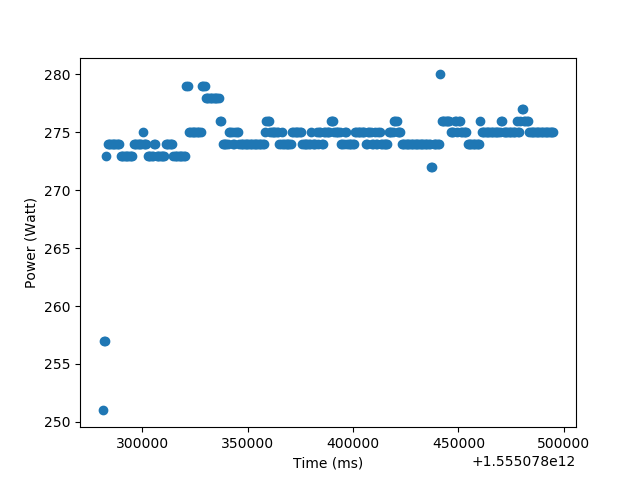
\includegraphics[width=.4\textwidth]{graphs/primesOpt.png}
    \caption{An example measurement of the primesOpt program.}
    \label{fig:primesOpt}
\end{figure}

An overview of the energy measurement set-up can be seen in figure \ref{fig:overview} and we created this set-up together with Stephan Kok. Here we can see that from the DAS-5 a job is sent to one of the energy measurement nodes. This is done by using the \textit{prun} command and specifying which node to use. The job we send to this node is a bash script that runs all the programs in our data set. In this job we sleep for ten seconds in between the measurements of the programs to give the node time to go back to its idle state. After these ten seconds the measure script on the DAS-4 is started and then the program we want to measure the energy consumption for starts to run on the node. Immediately after the program ends the measure script is stopped. This measure script on the DAS-4 constantly sends a \textit{snmp} message to the PDU and writes the values to an output file. Due to the other nodes constantly being occupied and the long run time, every program was able to run 27 times on \textit{node28} and 22 times on \textit{node29}.
%Only six nodes on the DAS-5 are connected to the PDU and all these nodes have different hardware specifications. Therefor we need to separate the measurements to be able to compare the results. Due to the other nodes constantly being occupied and the long run time, every program was able to run 27 times on \textit{node28} and 22 times on \textit{node29}. The hardware specifications for \textit{node28} are a GPU node with an Nvidia Tesla K20 (with 6 GB onboard memory), an Xeon Phi and a michost and for \textit{node29} are a GPU node with an Nvidia GTX980 (with 4 GB onboard memory) and an TitanX-Pascal.

% An overview of our set-up can be seen in figure \ref{fig:overview}. On the DAS-5 we have a run script which takes as one of its arguments a filename. This filename is the file we want to test for energy consumption. We run the run script with the command \textit{srun} and choose one of the nodes that is connected to the PDU. The first thing this script does is send a message to the DAS-4 to start the measurement, after this the program which corresponds to the filename is executed and when that is finished the script sends a message to the DAS-4 that the measurement can be stopped. When the DAS-4 receives the message to start measuring it will execute its measure script until it receives the stop message. This measure script constantly retrieves the data from the PDU and writes it to an output file. The files used for this set-up are in a public Git-Hub repository at \url{https://github.com/lukaskoedijk/Green-Software} in the \textit{EnergyMeasurement} folder.

\begin{figure}[h]
    \centering
    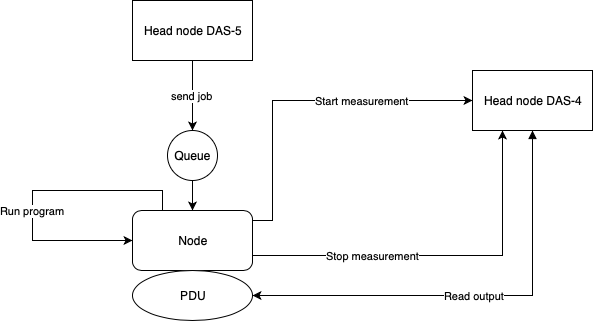
\includegraphics[width=.6\textwidth]{graphs/das.png}
    \caption{The structural overview of how we used the DAS to measure the energy consumption. From the head node of the DAS5 we send jobs to the queue of a certain node we want to measure on. This job will then run on that node when its available. In the job we send a message to the DAS4 to starts its energy measurement, then we run the programs and after that we send a message to the DAS4 to stop the energy measurement. The DAS4 retrieves the energy measurements from the PDU via constant smtp requests.}
    \label{fig:overview}
\end{figure}

Our script on the DAS-4 uses \textit{snmpwalk} to retrieve the values from the PDU. The time it takes to retrieve the data from the PDU using \textit{snmpwalk} is not constant. This means that we need to take into account that we have some loss of information and in some cases even too few measure points. When there are less then 30 energy measurements for a program, that specific programs will run again until it has enough measure points. In figure \ref{fig:time_diff} the average time between two measure points is shown alongside the standard deviation, the maximum and minimum time difference. There we can see that the average time between two measures is really fast, but the largest time period between two measures is really long. 

\begin{figure}[h]
    \centering
    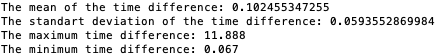
\includegraphics[width=.6\textwidth]{graphs/time_between_measures.png}
    \caption{Some statistics of the time between two energy measurement in seconds.}
    \label{fig:time_diff}
\end{figure}

%-talk about the difference in the nodes (hardware)
%-maybe about measure time diff
%TODO:
%-maybe something about scratch dir, no
\chapter{Data}
\label{ch:data}

\section{Programming languages}
To find data we first need to decide which programming languages to choose for testing. We did this by looking into what the most popular and most used programming languages are. For this question it depends who you ask which result you get. Therefor four sources were used to determine which programming language to use. The four sources are indeed, git-hub, TIOBE and PYPL.\\
%what the resulting most popular programming language is

Indeed is a job search site. They looked at the percentage of jobs with a programming language in their name in the tech software category \cite{ray:2018}. Thus the more job offering for a programming language the more popular that programming language is. The problem with this method is that job offerings do not show how many people work with a programming language, but only which programming language has a shortage in programmers. Based on data form September 2018 the top ten according to this method is Java, JavaScript, HTML, Python, C\#, C++, XML, Ruby, PHP and Perl.\\

Git-hub is a version control system where multiple programmers collaborate in a project. They looked at the amount of pull requests made for that language \cite{zap:2019}. The thought was that the language that programmers work a lot with on git is the most popular, but this is based on only the public repositories. In the first quarter of 2019 the top ten according to this method is JavaScript, Python, Java, Go, C++, Ruby, PHP, TypeScript, C\# and C. \\

TIOBE is a software quality company. They looked at the amount of hits they got when searching "[Language] programming" on a lot of different search engines \cite{tio:2019}. There are rules which a search engine needs to comply with for it to be used in the calculations and they also look a what type of hits they find to determine whether or not to use it in the calculations. The pitfall of this method is the favouritism for complex languages. When a language is more difficult to understand, more page of tutorials are needed and more questions about this language will be asked. As of April 2019 the top 10 according to this method is Java, C, C++, Python, Visual Basic .NET, C\#, JavaScript, SQL, PHP and Assembly language.\\

PYPL index stands for the PopularitY Programming Language index. They look at how many times a language tutorial is searched \cite{car:2019}. This method also has favouritism for complex languages, where programmers need to use the tutorials a lot because of the difficulty. Based on data form April 2019 the top ten according to this method is Python, Java, JavaScript, C\#, PHP, C/C++, R, Objective-C, Swift and Matlab.\\

When languages are in all the four top tens they were labelled as popular and these are the languages that are gonna be investigated, thus the languages Java, JavaScript, Python, C\#, C++ and PHP. We also choose to investigate C and Ruby. C because it was in three of the four top tens and it seemed interesting to see the difference in the variations of C like C++ and C\#. Ruby was in two of the top tens, but also 13th according to TIOBE and 12th in the PYPL index. Thus Ruby was close to be in all the top tens and therefor also chosen to be investigated.


% Binarytrees:
% -Java:
% 	-1 -> not correct output
% 	steps:
% 		- mv binarytrees.java-7.java binarytrees.java
% 		- javac -d . binarytrees.java
% 		- java binarytrees 21
% 		- rm -v binarytrees.class binarytrees\$1.class binarytrees\$TreeGenerator.class binarytrees\$TreeNode.class 		(just for clean up, but new javac overwrites these files)
%   das5:
%       -srun javac binarytrees.java && java binarytrees 21
%       -srun -N1 -w "node028" run_continues.sh  -o "test_java" -p "3" -f "javac -d /home/lkoedijk/binarytrees /home/lkoedijk/binarytrees/binarytrees.java,java -cp /home/lkoedijk/binarytrees/ binarytrees 21"
%
% 	java version local (java -version):
% 		- java version "1.8.0_191"
% 		- Java(TM) SE Runtime Environment (build 1.8.0_191-b12)
% 		- Java HotSpot(TM) 64-Bit Server VM (build 25.191-b12, mixed mode)
%     das5:
%         -openjdk version "1.8.0_161"
%         -OpenJDK Runtime Environment (build 1.8.0_161-b14)
%         -OpenJDK 64-Bit Server VM (build 25.161-b14, mixed mode)

% -Python:
%     steps:
%         -mv binarytrees.python3.py binarytrees.py
%         -python3 binarytrees.py 21
%     das5:
%         -srun -N1 -w "node028" run_continues.sh  -o "test_py" -p "3" -f "python3 /home/lkoedijk/binarytrees/binarytrees.python3.py 21"
        
%     python3 local version (python3 --version):
%         - Python 3.6.0 :: Anaconda custom (x86_64)
%     das5:
%         -Python 3.4.5
        
% -JavaScript:
%     steps:
%         -cp -L binarytrees.node binarytrees.js
%         -node binarytrees.js 21
%    das5:
%       -srun -N1 -w "node028" run_continues.sh  -o "test_javascript" -p "3" -f "node /home/lkoedijk/binarytrees/binarytrees.js 21"
        
%     javascript local version (node -v):
%         -v11.10.0
%     das5:
%         -v6.12.3
        
% -PHP:
%     -4, 5, 6 -> error: undefined function pcntl_fork()
%     steps:
%         -php -n -d memory_limit=4096M binarytrees.php 21
%     das5:
%         -srun -N1 -w "node028" run_continues.sh  -o "test_php" -p "3" -f "php -n -d memory_limit=4096M /home/lkoedijk/binarytrees/binarytrees.php 21" 
        
%     php local version (php -v):
%         -PHP 7.1.23 (cli) (built: Nov  7 2018 18:20:35) ( NTS )
%         -Copyright (c) 1997-2018 The PHP Group
%         -Zend Engine v3.1.0, Copyright (c) 1998-2018 Zend Technologies
%     das5:
%         -PHP 5.4.16 (cli) (built: Mar  7 2018 13:34:47) 
%         -Copyright (c) 1997-2013 The PHP Group
%         -Zend Engine v2.4.0, Copyright (c) 1998-2013 Zend Technologies
        
% -Ruby:
%     steps:
%         -ruby -W0 binarytrees.yarv 21
%     das5:
%         -srun -N1 -w "node028" run_continues.sh  -o "test_php" -p "3" -f "ruby -W0 /home/lkoedijk/binarytrees/binarytrees.yarv 21"
        
%     ruby local version (irb -> RUBY_VERSION -> exit):
%         -2.3.7
%     das5:
%         -2.0.0

% -C:
%     -3 -> error apr_pools.h not found
%     steps:
%         -/usr/bin/gcc -pipe -Wall -O3 -fomit-frame-pointer -march=native -I/usr/include/apr-1.0 binarytrees.gcc.c -o binarytrees.gcc_run -lapr-1
%         -./binarytrees.gcc_run 21
    % das5:
    %     -(for program 5)gcc -pipe -Wall -O3 -fomit-frame-pointer -march=native -I/usr/include/apr-1.0 -pthread binarytrees.gcc-5.c -o binarytrees.gcc_run
    %     -(for program 0)gcc -pipe -Wall -O3 -fomit-frame-pointer -march=native -I/usr/include/apr-1.0 /home/lkoedijk/binarytrees/binarytrees.gcc.c -o binarytrees.gcc_run -lm
    %     -(for program 3) need apr_pools.h
    %     -srun -N1 -w "node028" run_continues.sh  -o "test_c" -p "3" -f "/home/lkoedijk/binarytrees/binarytrees.gcc_run 21"
        
%     c local version (gcc -v):
%         -Configured with: --prefix=/Applications/Xcode.app/Contents/Developer/usr --with-gxx-include-dir=/Applications/Xcode.app/Contents/Developer/Platforms/MacOSX.platform/Developer/SDKs/MacOSX10.14.sdk/usr/include/c++/4.2.1
%         -Apple LLVM version 10.0.0 (clang-1000.11.45.5)
%         -Target: x86_64-apple-darwin18.2.0
%         -Thread model: posix
%         -InstalledDir: /Applications/Xcode.app/Contents/Developer/Toolchains/XcodeDefault.xctoolchain/usr/bin
%     das5:
%         -Using built-in specs.
%         -COLLECT_GCC=gcc
%         -COLLECT_LTO_WRAPPER=/cm/local/apps/gcc/6.3.0/libexec/gcc/x86_64-pc-linux-gnu/6.3.0/lto-wrapper
%         -Target: x86_64-pc-linux-gnu
%         -Configured with: ../gcc-6.3.0/configure --prefix=/cm/local/apps/gcc/6.3.0 --enable-languages=c,c++,fortran --with-gmp-include=/root/rpmbuild/BUILD/gcc-6.3.0-obj/../gcc-6.3.0/our-gmp --with-gmp-lib=/root/rpmbuild/BUILD/gcc-6.3.0-obj/../gcc-6.3.0/our-gmp/.libs --with-mpc-include=/root/rpmbuild/BUILD/gcc-6.3.0-obj/../gcc-6.3.0/our-mpc/src --with-mpc-lib=/root/rpmbuild/BUILD/gcc-6.3.0-obj/../gcc-6.3.0/our-mpc/src/.libs --with-mpfr-include=/root/rpmbuild/BUILD/gcc-6.3.0-obj/../gcc-6.3.0/our-mpfr/src --with-mpfr-lib=/root/rpmbuild/BUILD/gcc-6.3.0-obj/../gcc-6.3.0/our-mpfr/src/.libs
%         -Thread model: posix
%         -gcc version 6.3.0 (GCC) 
        
% c++:
%     -2,6 -> wrong answers
%     -9 -> missing apr_pools.h
%     steps:
%         -(for 1,3)g++ -c -pipe -O3 -fomit-frame-pointer -march=native /home/lkoedijk/binarytrees/binarytrees.gpp-3.c++ -o /home/lkoedijk/binarytrees/binarytrees.gpp.c++.o && g++ /home/lkoedijk/binarytrees/binarytrees.gpp.c++.o -o /home/lkoedijk/binarytrees/binarytrees.gpp_run -lpthread -lboost_system
%         -(for 8)g++ -c -pipe -O3 -fomit-frame-pointer -march=native -fopenmp /home/lkoedijk/binarytrees/binarytrees.gpp-8.c++ -o /home/lkoedijk/binarytrees/binarytrees.gpp.c++.o && g++ /home/lkoedijk/binarytrees/binarytrees.gpp.c++.o -o /home/lkoedijk/binarytrees/binarytrees.gpp_run -lboost_system -fopenmp
%         -./binarytrees.gpp_run 21

    % fannkuchredux:
    %     -2,3,5 error
    
%     c++ local version (g++ -v):
%         -Configured with: --prefix=/Applications/Xcode.app/Contents/Developer/usr --with-gxx-include-dir=/Applications/Xcode.app/Contents/Developer/Platforms/MacOSX.platform/Developer/SDKs/MacOSX10.14.sdk/usr/include/c++/4.2.1
%         -Apple LLVM version 10.0.0 (clang-1000.11.45.5)
%         -Target: x86_64-apple-darwin18.2.0
%         -Thread model: posix
%         -InstalledDir: /Applications/Xcode.app/Contents/Developer/Toolchains/XcodeDefault.xctoolchain/usr/bin
%     das5:
%         -Using built-in specs.
%         -COLLECT_GCC=g++
%         -COLLECT_LTO_WRAPPER=/cm/local/apps/gcc/6.3.0/libexec/gcc/x86_64-pc-linux-gnu/6.3.0/lto-wrapper
%         -Target: x86_64-pc-linux-gnu
%         -Configured with: ../gcc-6.3.0/configure --prefix=/cm/local/apps/gcc/6.3.0 --enable-languages=c,c++,fortran --with-gmp-include=/root/rpmbuild/BUILD/gcc-6.3.0-obj/../gcc-6.3.0/our-gmp --with-gmp-lib=/root/rpmbuild/BUILD/gcc-6.3.0-obj/../gcc-6.3.0/our-gmp/.libs --with-mpc-include=/root/rpmbuild/BUILD/gcc-6.3.0-obj/../gcc-6.3.0/our-mpc/src --with-mpc-lib=/root/rpmbuild/BUILD/gcc-6.3.0-obj/../gcc-6.3.0/our-mpc/src/.libs --with-mpfr-include=/root/rpmbuild/BUILD/gcc-6.3.0-obj/../gcc-6.3.0/our-mpfr/src --with-mpfr-lib=/root/rpmbuild/BUILD/gcc-6.3.0-obj/../gcc-6.3.0/our-mpfr/src/.libs
%         -Thread model: posix
%         -gcc version 6.3.0 (GCC) 

%C#:
%   steps:
%       -mcs binarytrees.cs
%       -srun -N1 -w "node028" run_continues.sh  -o "test_c" -p "3" -f "mono /home/lkoedijk/binarytrees/binarytrees.exe 21"


%!!!!Knucleotide error with only javascript file, different error local and on das
%!!!!Knucleotide error with only c file, no khash.h file
%!!!!Pidigits all three python files, No module named 'gmpy'
%!!!!Regexredux php with error, Call to undefined function msg_get_queue()
%!!!!Regexredux c++ 1,2,5: fatal error: 're2/re2.h' file not found
%               c++ 4:fatal error: string_view: No such file or directory

\section{Gathering data}
To be able to compare different programs they need to have the same functionality. A source for programs that have the same functionality is  \textit{the computer language benchmark game} \cite{gouy:2019}. This benchmark game compares different programs and languages based on their speed, memory usage, zipped program size and CPU usage. They have ten different problems with a lot of programs from different languages. Everyone can submit a program if it holds to the two requirements. The requirements are that the program has the correct output and that it uses the same algorithm. This is important because we want to compare the way of writing a program and the difference in programming language, but not the difference in algorithm used. For every program used they also have the compiling steps listed and for every problem the correct output.\\

All the programs for the ten problems in our seven programming languages were downloaded. These programs were then tested to see if they could compile, run and have the correct output. This was all done on the DAS5 to make sure there were no local dependencies. All the programs that weren't compiling, gave a run error or gave the wrong output were excluded from the data set. There were three problems, Knucleotide, Pidigits and Regexredux, that for different programming languages use a partly different algorithm because of different library implementations. Therefor we excluded these problems from the data set. The problem Mandelbrot didn't have a working version of the JavaScript implementation, but this problem will still be used and we will just have an empty spot in our results.\\

% that didn't had for every programming language a program that could be run or had the correct output and they also had . I decided to still run these problems and just have a few empty slot in our results. For Knucleotide the programming languages were JavaScript and C, for Regexredux it was PHP and C++ and for Pidigits it was Python3. I have this data set on a public Git-Hub repository along side other material needed for my thesis. The link to this repository is \url{https://github.com/lukaskoedijk/Green-Software} and for the data set move to \textit{EnergyMeasurement/programs}.\\

Before running all the programs some needed to be compiled first. The compilation step of languages that have a separated compilation step were not included in the energy measuring. The reason for this is that a finished program is compiled once and then could be used multiple times. This does mean that the languages JavaScript, Python, PHP and Ruby have a bit of a disadvantage, because they don't have a separate compilation step. The compiler can nowadays do a lot of optimizations of the code. During this research we want to see the result of user decisions on the energy consumption. Therefore besides testing the programs with the flags used on the language benchmark game we also tested with as few flags as possible. This means that we removed all the optimization flags except the ones needed for the compilation. Also the compiler version of the different languages is important. To give a good pictures of were we stand today we need to use the most recent stable version and also the most commonly used one. Unfortunately it isn't that easy to update the language versions on the DAS. Therefore I used the versions that were already on their and these programming language versions are listed alongside the compiler used in table \ref{tab:version}.

\begin{table}[h]
\centering
\begin{tabular}{|l|l|l|}
\hline
\textbf{Languages}  & \textbf{Compiler} & \textbf{Version}   \\ \hline
Java       & javac    & 1.8.0\textunderscore161 \\ \hline
JavaScript & node     & 6.12.3    \\ \hline
Python     & python   & 3.4.5     \\ \hline
PHP        & php      & 5.4.16    \\ \hline
C          & gcc      & 6.3.0     \\ \hline
C++        & gcc      & 6.3.0     \\ \hline
C\#         & mcs      & 5.10.1.20 \\ \hline
Ruby       & ruby     & 2.0.0     \\ \hline
\end{tabular}
\caption{All the different compilers and versions of the programming languages used}
\label{tab:version}
\end{table}

This all resulted in a large data set of 202 programs with 67 programs that had to run twice, once with and once without flags. Running all these programs takes about eight hours to complete. Unfortunately we were only allowed to use a node on the DAS for 30 minutes to run one script during working hours. This means that we had to run it at night and in the weekend, which limited the amount of data points that were measured. Of course running programs more often would give more accurate results, but this was just too time consuming.\\

Some programs were too fast to get a good amount of energy measurement points. To solve this problem those programs were run for multiple times during one measurement and then afterwards their energy consumption was divided by the amount of times the programs was run. Another problem that occurred was that retrieving a measure point takes a variable amount of time. This caused some programs to still not have a good amount of energy measurement points. Therefor I decided to set a minimum amount of 30 of measurement points needed in order for it to be used. \\
% With data from the benchmark game I calculated that to run all the programs for the eight programming languages for the ten problems would take around nine hours. Because this is a large amount of time I decided to only measure every program three times, which would take around 27 hours. Of course running programs more often would give more accurate results, but this was just too time consuming.\\

% PHP:-d memory_limit=1024M -> set entry memory_limit to 1024M
% C:  -pipe -> use pipe instead of temporary files for communication                     between compiling stages 
%     -Wall -> turn on multiple warning flags
%     -O3 -> turns on a lot of optimization flags
%     -fomit-frame-pointer -> optimization, Omit the frame pointer in                            functions that don’t need one
%     -march=native -> pick the architecture of the host system
%     -lm -> link math library
%     (-lapr-1 -> link apr-1 library)
%     (-lgomp -> link gomp library)
%     -fopenmp -> enable handling of OpenMP directives(multithreading)
%     -D_FILE_OFFSET_BITS=64 -> this forces all file access calls to use                             the 64 bit variants
%     -I/usr/include/apr-1.0 -> specify directory to search for header                               files
%     -pthread -> define additional macros required for using the POSIX              threads library
%     -IInclude -> ?
%     -mno-fma -> enable the use of instructions in the no-fma instruction              set
%     -fno-finite-math-only -> ?
%     -lgmp -> link gmp library
%     -lpcre -> link pcre library
% c++:
%     -c -> compile or assemble the source files, but do not link
%     -lpthread -> link pthread library
%     -std=c++11(c++14) -> determine the language standard
%     -lboost_thread -> link boost_thread library
%     -lboost_system -> link boost_system library
%     -mfpmath=sse -> generate floating-point arithmetic for sse
%     -msse3 -> enable the use of instructions in the MSSE3 instruction              set
%     -Wl,--no-as-needed -> pass option no as needed to linker?
%     -lgmpxx -> link gmpxx library
%     -flto -> runs the standard link-time optimizer
%     -mtune=native -> specify the name of the target processor for which                     GCC should tune the performance of the code
%     -O0 -> disable optimizations
% Ruby: -w0 -> verbose mode silence

In the previous chapter we found that the energy consumption of a program is the sum of the CPU, memory and disk energy consumption \cite{acar2016impact}. To get a good view on what influences the energy consumption, our problems need to be diverse when it comes to these three categories. The problems that we looked into are called Binarytrees, Fannkuchredux, Fasta, Mandelbrot, Nbody, Revcomp and Spectralnorm. For the Binarytrees problem a lot of trees are allocated and deallocated in memory and thus this is a memory intensive task. The fannkuchredux problem does a lot of calculations on all permutations and is thus CPU intensive. The Fasta problem creates and saves a large DNA sequence and is memory intensive. For the Mandelbrot problem a large bitmap is saved and thus is it memory intensive. The Nbody problem models the orbit of Jovian planets and is CPU intensive. The Revcomp problem reads a DNA sequences line by line, transforms them and writes the result to output. Therefor the Revcomp problem is disk intensive. For the Spectralnorm problem a lot of calculations are done on a large matrix and is thus CPU intensive. A more extensive explanation of the problems can be found on the computer language benchmark game website \cite{gouy:2019}. An overview of category and problem is shown in table \ref{tab:problems}.

\begin{table}[h]
\centering
\begin{tabular}{|l|l|}
\hline
\textbf{Category} & \textbf{Problems}                           \\ \hline
CPU      & Fannkuchredux, Nbody, Spectralnorm \\ \hline
Memory   & Binarytrees, Fasta, Mandelbrot     \\ \hline
Disk     & Revcomp                            \\ \hline
\end{tabular}
\caption{The job intensive categories the different problems are in}
\label{tab:problems}
\end{table}

% tell which problem is I/O(disk?), memory or CPU insensitive
% description of problems can be found on site
% spectral-norm(maybe memory), n-body(maybe cpu)
% cpu(mainly calculations): fannkuchredux
% memory(lot of data stored or large data stored):mandelbrot, fasta, rev-comp, binarytrees (allocate/deallocate)
% disk: fasta, rev-comp

% pidigits*(maybe memory), regex-redux*(memory maybe disk), knucleotide*(memory and disk)

% minimal run time of 7 seconds to get a good amount of datapoints, 0.6-0.7 seconds per measure thus like 10 datapoint minimal, the more the better but we have not that much time

%-talk about amount of files and runtime of single run of all programs
%-talk about runtime (7 seconds)
%-talk about the reason programs/problems do not work and are leftout
%-tell that the versions are this version because these were on the das
%-talk about different types of problems (cpu, memory, disk)
%-talk about compilation (flags, pre-compilation), why not measured
%TODO:

\chapter{Results}
\label{ch:results}
In this chapter, we present the results of our experiment. 

table with languages
table with programs averages
figure per problem
example figure of a problem with different programs in same language
anomalies
same distribution

without flags, takes more energy

For binarytrees: php cosumes the most, python ruby and csharp also relatively bad 
For fannkuchredux: php python ruby really bad, javascript also not so good
For fasta: php python ruby javascript not good
For mandelbrot: python php ruby not good
For nbody: python php ruby not good
For revcomp: not one that really stands out, though c++-noflags has a huge range thus potentially really bad
For spectralnorm: python least good, php ruby also not good

Overall php, python and ruby not good conform the energy consumption
\chapter{Discussion}
\label{ch:discussion}
In this chapter, we discuss the results of our experiment(s) on ...

\begin{finding}
	Highlight like this an important finding of your analysis of the results.
	\label{find:important1}
\end{finding}

Refer to Finding~\ref{find:important1}.



Risks:
-compiler maybe expects people to program stupidly
\chapter{Related work}
\label{ch:related_work}
%We divide the related work into ... categories:  ...
%-overview
%-subsection{finding optimal energy consumption}
%-subsection{estimating energy consumption}
%-subsection{hardware influence on energy consumption}
%-subsection{software influence on energy consumption}
%-subsection{other}

To get an overview of the related research we made the table \ref{table:LiteratureStudy} where we are comparing different related papers. Most research is about reducing the energy consumption of a specific piece of hardware, for example scheduling on a multi-core processor. There are also some papers about reducing the energy consumption in the software and the decision making process. There is also some research done on the energy consumption of software, but their research goal was to estimate the energy consumption. 
%Therefore what I miss and want to look into is to research if there is a good way of writing code regards the energy consumption.

\begin{table}[h]
\resizebox{\textwidth}{!}{%
\begin{tabular}{|l|l|l|l|}
\hline
\textbf{Papers}& \textbf{Type of Research} & \textbf{Unit of Analysis} & \textbf{Goal} \\ \hline
\cite{verdecchia2017estimating} & Controlled Experiment & \begin{tabular}[c]{@{}l@{}}Deployment strategies, \\ releases and use case scenarios\end{tabular} & Finding optimal energy consumption \\ \hline
\cite{filip2015bats} & \begin{tabular}[c]{@{}l@{}}Case Study \&\\ Controlled Experiment\end{tabular} & HPC bag of task applications & Finding optimal energy consumption \\ \hline
\cite{acar2016impact} & Case Study & Small functions & Estimating energy consumption \\ \hline
\cite{liqat2013energy} & \begin{tabular}[c]{@{}l@{}}Case Study \&\\ Controlled Experiment\end{tabular} & Small functions & Estimating energy consumption \\ \hline
\cite{jayaseelan2006estimating} & Case Study & Task on complex micro-architectures & Estimating worst-case energy consumption \\ \hline
\cite{ferreiradasilva-iccs-2019} & Controlled experiment & I/O application tasks &  Estimating energy consumption of I/O tasks\\ \hline
\cite{sahin2014code} & Empirical Study & Six commonly used refactorings & \begin{tabular}[c]{@{}l@{}}Finding impact of refactorings\\ on energy consumption\end{tabular} \\ \hline
\cite{pereira2017energy} & Controlled experiment & Programming languages & \begin{tabular}[c]{@{}l@{}}Rank programming languages based on \\speed, memory usage and energy consumption\end{tabular} \\ \hline
\cite{zakarya2013energy} & Case Study & Multi-core processor scheduling & Efficient workload partitioning \\ \hline
\cite{zhu2004reducing} & Case Study & Cache storage management algorithms & Power aware cache management\\ \hline
\cite{manotas2014seeds} & Case Study & Java applications & \begin{tabular}[c]{@{}l@{}}Framework to automate decision-making\\ support regarding energy consumption\end{tabular} \\ \hline
\cite{mahmoud2013green} & Case Study & Software process & Two level green software model \\ \hline

\end{tabular}%
}
\caption{Overview of related research}
\label{table:LiteratureStudy}
\end{table}

%1 and 2
\section{Finding optimal energy consumption}
The paper \cite{verdecchia2017estimating} looks at the impact of releases and deployment strategies of a software product on the energy consumption. They used a controlled experiment where the variables they changed where deployment strategies, releases and use case scenarios. The variables they measured during their tests were power consumption and execution time. They saw that both the releases and deployment strategies impacted the energy consumption and that this impact was influenced by which use case scenario they used. Therefore they concluded that there is no absolute optimal option for releases and deployment strategies with respect to energy consumption. They also found that the execution time had a bigger impact on the energy consumption than the power consumption, because of the low variability in power consumption.\\

The paper \cite{filip2015bats} looks at the scheduling of bags of task application in High performance Computing (HPC). They delved into the trade-off between energy consumption and performance by finding a optimal point for both variables. This was calculated by designing a dynamic Hill Climbing algorithm. Their algorithm uses less then 12\% of the resources an exhausted search would use to find a majority of points close to the optimal for the trade-off in 10 of the 12 scenarios. They validated their algorithm by implementing it and running a wide range of HPC bag of task applications. They found that the estimations of their algorithm have an error below 5\%.\\

%3, 4 and 5 
\section{Estimating energy consumption}
The paper \cite{acar2016impact} looks at different techniques to measure the power consumption. Then they propose a model to measure the power consumption and they used this model in their implementation named \textit{Tool to Estimate Energy Consumption} (TEEC). They test their implementation against a power meter, but they do not mention how accurate their implementation is. The figure they use at the validation is also not clear, they just state that it shows the same behaviour as TEEC. They find that the power consumption of unoptimized code is higher and has a longer execution time than the optimized code. They do not mention it, but looking at their graphs the unoptimized and optimized code seem to have the same peaks where the only difference is the time steps and that the optimized code is faster.\\

The paper \cite{liqat2013energy} estimates the energy consumption by developing a model which can be applied at instruction set simulation level. This was done by designing a translation from instruction set architecture code to Horn-clause representation and this model is called in the paper \textit{Instruction Set Simulation} (ISS). They also use the CiaoPP general resource analysis framework, which is low level, to model the energy consumption. They named it \textit{Static Resource Analysis} (SRA) in the paper. In their experiments they only use small functions to test and the results were compared to a mathematical equation. They found that the ISS function is less accurate when the value of N increases and that the SRA function is not accurate for small values of N. Here N is the input value of the function that is tested for its energy consumption.\\

%TODO: STILL NEED TO REREAD AND ADD HOW THEY ESTIMATE
The paper \cite{jayaseelan2006estimating} estimates the worst-case energy consumption of a task on complex micro-architectures. This is important for battery-operated embedded devices, where we don't what the battery to drain empty before a critical task is completed. They test their result against a commonly used benchmark and they find that their values have at most 33\% difference with the benchmark.\\

%Evaluation on the same application as used for calculating this new equation
The paper \cite{ferreiradasilva-iccs-2019} looks at two applications that are I/O heavy. Different tasks were run for these applications and the energy consumption was measured. Another variable in their experiments was the amount of cores used. They compared the energy values measured with a commonly used estimation scheme for the energy consumption which only looks at the CPU utilization. They noticed a difference in energy consumption and the correlation between power consumption and CPU utilization was close to zero. The reason for this was that the estimation scheme didn't factor in the energy consumption of I/O operations. Therefor they came up with a scheme that factors in the CPU utilization and the I/O operations. This scheme used values from the tests to put in different values in the formula and was tested against the two applications and they found a small error. This is an issue, because you expect the data you used to create a model to fit the model. A better approach would have been to use one application for calculating the values and the other for the validation.\\

%6 and 7
\section{Measuring energy consumption}
%Mann-Whitney-Wilcoxon to see if statistically significant difference
The paper \cite{sahin2014code} addresses the lack of information about the energy impact of code refactorings. They did this by testing the energy impact of 197 projects when the using six commonly used refactorings. From this test they found that refactorings can influence the energy consumption. Also they find that one refactoring does not necessarily have the same influence on the energy consumption when used with different projects.\\

The paper \cite{pereira2017energy} tries to find a connection between the speed, memory usage and energy consumption of a programming language. They do this by choosing the fastest implementation of the exact same algorithm, defined in the computer language benchmarks game, in different programming languages. From these programs they measured the execution time, memory usage and energy consumption. They used Intel’s Running Average Power Limit (RAPL) tool to measure the energy consumption and for the memory usage and execution speed they used the \textit{time} command available in Unix-based systems. They find that a faster programming language does not necessarily have a lower energy consumption and memory usage does not relate to energy consumption. A big problem with this paper is that in their threads to validity paragraph they defend their implementation instead of stating what could be wrong with their implementation.\\
%Another problem with this paper is that they compare languages based on the fastest solution in some competition and these are not comparable. Because there can be languages where the fastest solution given in the competition is not the fastest at all.\\

%8 and 9
\section{Hardware}
The paper \cite{zakarya2013energy} proposes an algorithm to makes sure all cores in a multi-core processor have the same workload. This is reducing energy consumption because multiple single core processors consume more energy.\\

The paper \cite{zhu2004reducing} tries multiple algorithms for storage cache management to decrease the energy consumption. One algorithm is an offline greedy algorithm and they also propose an online algorithm. They evaluate their algorithms by simulating a complete storage system, enhancing the DiskSim simulator. Their greedy algorithm results in 16\% less energy used then the LRU algorithm. They also find that the cache policy write-back can use 20\% less energy then write-through.\\

%10 and 11
\section{Other}
The paper \cite{manotas2014seeds} implements a framework that automatically optimizes the energy consumption of a Java software project. The framework does this by running multiple different given options and testing which option consumes the least amount of energy. Thus as input the framework needs a list of possible changes. Because the framework needs possible changes we don't know if the resulting code is the most energy efficient version, only that it is more energy efficient then the other input. They showed that by letting their framework chose which library to use they reduced their energy consumption by 17\%.\\

The paper \cite{mahmoud2013green} makes a two level green software model. The first level is about making the software process more energy efficient. This new process is a hybrid of the sequential, iterative, and agile development processes. The second level is about the role software tools can have on improving the energy efficiency of software. They also discus the relationship between the two levels.\\


% \subsection{Estimating energy impact of software releases and deployment strategies: the KPMG case study \cite{verdecchia2017estimating}}
% This paper looks at the impact of releases and deployment strategies of a software product on the energy consumption. They used a controlled experiment where the variables they changed where deployment strategies, releases and use case scenarios. The variables they measured during their tests were power consumption and execution time. They saw that both the releases and deployment strategies impacted the energy consumption and that this impact was influenced by which use case scenario they used. Therefore they concluded that there is no absolute optimal option for releases and deployment strategies with respect to energy consumption. They also found that the execution time had a bigger impact on the energy consumption than the power consumption, because of the low variability in power consumption.

% \subsection{The Impact of Source Code in Software on Power Consumption \cite{acar2016impact}}
% This paper looks at different techniques to measure the power consumption. Then they propose a model to measure the power consumption and they used this model in their implementation named \textit{Tool to Estimate Energy Consumption} (TEEC). They test their implementation against a power meter, but they do not mention how accurate their implementation is. The figure they use at the validation is also not clear, they just state that it shows the same behaviour as TEEC. They find that the power consumption of unoptimized code is higher and has a longer execution time than the optimized code. They do not mention it but looking at their graphs, the unoptimized and optimized code seem to have the same peaks only on different time steps for the optimized code is faster.

% \subsection{Energy Consumption Analysis of Programs based on XMOS ISA-Level Models \cite{liqat2013energy}}
% This paper estimates the energy consumption by developing a model which can be applied at instruction set simulation level. This was done by designing a translation from instruction set architecture code to Horn- clause representation and this model is called in the paper \textit{Instruction Set Simulation} (ISS). They also use the CiaoPP general resource analysis framework, which is low level, to model the energy consumption. They named it \textit{Static Resource Analysis} (SRA) in the paper. In their experiments they only use small functions to test and the results were compared to a mathematical equation. The found that the ISS function is less accurate when the value of N increases and that the SRA function is only not accurate for small value of N. Here N is the input value of the function that is tested for its energy consumption.

% \subsection{E-BATS: ENERGY-AWARE SCHEDULING FOR BAG-OF-TASK APPLICATIONS IN HPC CLUSTERS \cite{filip2015bats}}
% This paper looks at the scheduling of bags of task application in High performance Computing (HPC). They delved into the trade-off between energy consumption and performance by finding a optimal point for both variables. This was calculated by designing a dynamic Hill Climbing algorithm. Their algorithm uses less then 12\% of the resources an exhausted search would use to find a majority of points close to the optimal for the trade-off in 10 of the 12 scenarios. They validated their algorithm by implementing it and running a wide range of HPC bag of task applications. They found that the estimations of their algorithm have an error below 5\%.

% \subsection{SEEDS: A Software Engineer’s Energy-Optimization Decision Support Framework \cite{manotas2014seeds}}
% This paper implements a framework that automatically optimizes the energy consumption of a Java software project. The framework does this by running multiple different given options and testing which option consumes the least amount of energy. Thus as input the framework needs a list of possible changes. Because the framework needs possible changes we don't know if the resulting code is the most energy efficient version, only that it is more energy efficient then the input. They showed that by letting their framework chose which library to use they reduced their energy consumption by 17\%.

%Mann-Whitney-Wilcoxon to see if statistically significant difference
% \subsection{How Do Code Refactorings Affect Energy Usage? \cite{sahin2014code}}
% This paper addresses the lack of information about the energy impact of code refactorings. They did this by testing the energy impact of 197 projects when the using six commonly used refactorings. From this test they found that refactorings can influence the energy consumption. Also they find that one refactoring does not necessarily have the same influence on the energy consumption when used with different projects.


% \subsection{Reducing Energy Consumption of Disk Storage Using Power-Aware Cache Management \cite{zhu2004reducing}}
% This paper tries multiple algorithms for storage cache management to decrease the energy consumption. One algorithm is an offline greedy algorithm and they also propose an online algorithm. They evaluate their algorithms by simulating a complete storage system, enhancing the DiskSim simulator. Their greedy algorithm results in 16\% less energy used then the LRU algorithm. They also find that the cache policy write-back can use 20\% less energy then write-through.



% \subsection{A Green Model for Sustainable Software Engineering \cite{mahmoud2013green}}
% This paper makes a two level green software model. The first level is about making the software process more energy efficient. This new process is a hybrid of the sequential, iterative, and agile development processes. The second level is about the role software tools can have on improving the energy efficiency of software. They also discus the relationship between the two levels.


% \subsection{Estimating the Worst-Case Energy Consumption of Embedded Software \cite{jayaseelan2006estimating}}
% This paper estimates the worst-case energy consumption of a task on complex micro-architectures. This is important for battery-operated embedded devices, where we don't what the battery to drain empty before a critical task is completed. They test their result against a commonly used benchmark and they find that their values have at most 33\% difference with the benchmark.

% \subsection{Energy Efficient Workload Balancing Algorithm for Real-Time Tasks over Multi-Core \cite{zakarya2013energy}}
% This paper proposes an algorithm to makes sure all cores in a multi-core processor have the same workload. This is reducing energy consumption because multiple single core processors consume more energy.

% \subsection{Energy Efficiency across Programming Languages
%  \cite{pereira2017energy}}
%  This paper tries to find a connection between the speed, memory usage and energy consumption of a programming language. They do this by choosing the fastest implementation of the exact same algorithm, defined in the computer language benchmarks game, in different programming languages. From these programs they measured the execution time, memory usage and energy consumption. They used Intel’s Running Average Power Limit (RAPL) tool to measure the energy consumption and for the memory usage and execution speed they used the \textit{time} command available in Unix-based systems. They find that a faster programming language does not necessarily have a lower energy consumption and memory usage does not relate to energy consumption. A big problem with this paper is that in their threads to validity paragraph they defend their implementation instead of stating what could be wrong with their implementation. My main problem with this paper is that they compare languages based on the fastest solution in some competition and these are not comparable. Because there can be languages where the fastest solution given in the competition is not the fastest at all.
 
 %  negative correlation factor?
%  Evaluation on the same application as used for calculating this new equation
%  \subsection{Accurately Simulating Energy Consumption of I/O-intensive Scientific Workflows \cite{ferreiradasilva-iccs-2019}}
%  This paper looks at two applications that are I/O heavy. Different tasks were run for these applications and the energy consumption was measured. Another variable in their experiments was the amount of cores used. They compared the energy values measured with a commonly used estimation scheme for the energy consumption which only looks at the CPU utilization. They noticed a difference and the correlation between power consumption and CPU utilization was close to zero. The reason for this was that the estimation scheme didn't factor in the energy consumption of I/O operations. Therefor they came up with a scheme that factors in the CPU utilization and the I/O operations. This scheme used values from the tests to put in different values in the formula and was tested against the two applications and they found a small error. This is an issue for me, because you expect the data you used to create a model to fit the model. A better approach would have been to use one application for calculating the values and the other for the validation.
 

\chapter{Conclusion}
\label{ch:conclusion}



\section{Future work}
\label{sec:future_work}

\chapter*{Acknowledgements}
If so inclined, thank people.
Kees Verstoep

\printbibliography[heading=bibintoc]
\printglossaries%

\begin{appendices}
	
\chapter{Node28}
\label{app:node28}
\begin{figure}[h]
    \centering
    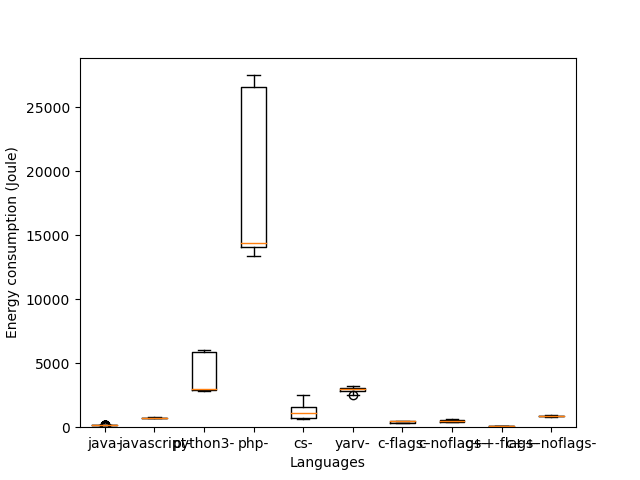
\includegraphics[width=.6\textwidth]{graphs/binarytrees_BOXoverview3.png}
    \caption{The box plot of the different programs in a programming language for the problem Binarytrees on \textit{node28}.}
    \label{fig:box-binarytrees3}
\end{figure}

\begin{table}[h]
\centering
\resizebox{\textwidth}{!}{%
\begin{tabular}{|l|c|c|c|c|c|c|c|c|c|c|}
\hline
 & \multicolumn{1}{l|}{Java} & \multicolumn{1}{l|}{JavaScript} & \multicolumn{1}{l|}{Python} & \multicolumn{1}{l|}{PHP} & \multicolumn{1}{l|}{C\#} & \multicolumn{1}{l|}{Ruby} & \multicolumn{1}{l|}{C-flags} & \multicolumn{1}{l|}{C-noflags} & \multicolumn{1}{l|}{C++-flags} & \multicolumn{1}{l|}{C++-noflags} \\ \hline
Java & 0 & + & + & + & + & + & + & + & - & +\\ \hline
JavaScript & - & 0 & + & + & + & + & - & - & - & +\\ \hline
Python & - & - & 0 & + & - & - & - & - & - & -\\ \hline
PHP & - & - & - & 0 & - & - & - & - & - & -\\ \hline
C\# & - & - & + & + & 0 & + & - & - & - & -\\ \hline
Ruby & - & - & + & + & - & 0 & - & - & - & -\\ \hline
C-flags & - & + & + & + & + & + & 0 & + & - & +\\ \hline
C-noflags & - & + & + & + & + & + & - & 0 & - & +\\ \hline
C++-flags & + & + & + & + & + & + & + & + & 0 & +\\ \hline
C++-noflags & - & - & + & + & + & + & - & - & - & 0\\ \hline
\end{tabular}%
}
\caption{The comparison of the different languages for the Binarytrees problem on \textit{node28}. A \textit{+} means that the language on the row has a lower energy consumption then the language on the column, the opposite for \textit{-}.}
\label{tab:lang-binarytrees3}
\end{table}

\begin{figure}[h]
    \centering
    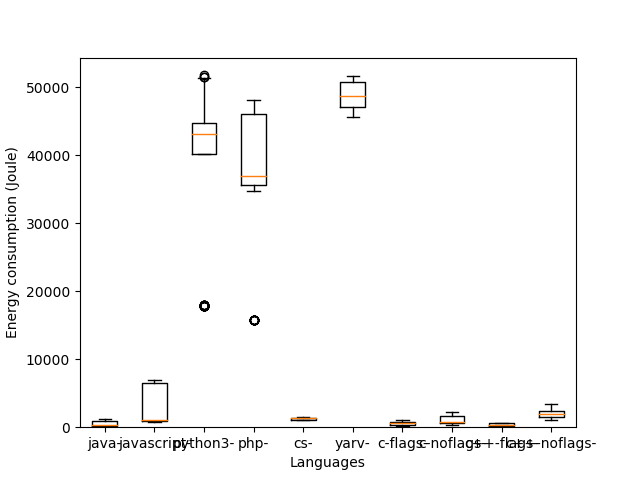
\includegraphics[width=.6\textwidth]{graphs/fannkuchredux_BOXoverview3.png}
    \caption{The box plot of the different programs in a programming language for the problem Fannkuchredux on \textit{node28}.}
    \label{fig:box-fannkuchredux3}
\end{figure}

\begin{table}[h]
\centering
\resizebox{\textwidth}{!}{%
\begin{tabular}{|l|c|c|c|c|c|c|c|c|c|c|}
\hline
 & \multicolumn{1}{l|}{Java} & \multicolumn{1}{l|}{JavaScript} & \multicolumn{1}{l|}{Python} & \multicolumn{1}{l|}{PHP} & \multicolumn{1}{l|}{C\#} & \multicolumn{1}{l|}{Ruby} & \multicolumn{1}{l|}{C-flags} & \multicolumn{1}{l|}{C-noflags} & \multicolumn{1}{l|}{C++-flags} & \multicolumn{1}{l|}{C++-noflags} \\ \hline
Java & 0 & + & + & + & + & + & + & + & + & + \\ \hline
JavaScript & - & 0 & + & + & + & + & - & - & - & + \\ \hline
Python & - & - & 0 & - & - & + & - & - & - & - \\ \hline
PHP & - & - & + & 0 & - & + & - & - & - & - \\ \hline
C\# & - & - & + & + & 0 & + & - & - & - & +\\ \hline
Ruby & - & - & - & - & - & 0 & - & - & - & -\\ \hline
C-flags & - & + & + & + & + & + & 0 & + & - & +\\ \hline
C-noflags & - & + & + & + & + & + & - & 0 & - & +\\ \hline
C++-flags & - & + & + & + & + & + & + & + & 0 & +\\ \hline
C++-noflags & - & - & + & + & - & + & - & - & - & 0\\ \hline
\end{tabular}%
}
\caption{The comparison of the different languages for the Fannkuchredux problem on \textit{node28}. A \textit{+} means that the language on the row has a lower energy consumption then the language on the column, the opposite for \textit{-}.}
\label{tab:lang-fannkuchredux3}
\end{table}

\begin{figure}[h]
    \centering
    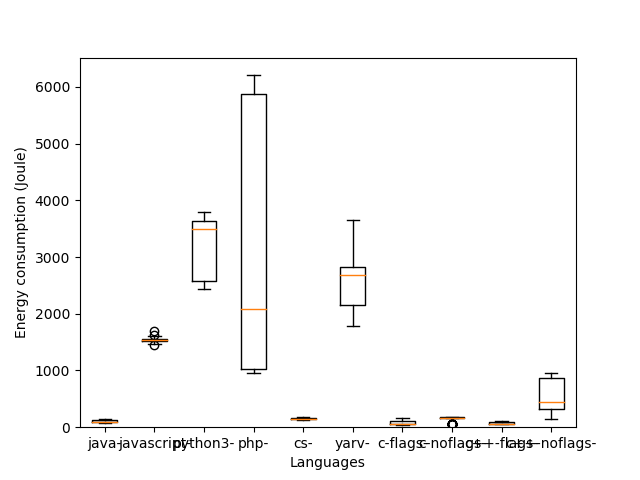
\includegraphics[width=.6\textwidth]{graphs/fasta_BOXoverview3.png}
    \caption{The box plot of the different programs in a programming language for the problem Fasta on \textit{node28}.}
    \label{fig:box-fasta3}
\end{figure}

% Please add the following required packages to your document preamble:
% \usepackage{graphicx}
\begin{table}[h]
\centering
\resizebox{\textwidth}{!}{%
\begin{tabular}{|l|c|c|c|c|c|c|c|c|c|c|}
\hline
 & \multicolumn{1}{l|}{Java} & \multicolumn{1}{l|}{JavaScript} & \multicolumn{1}{l|}{Python} & \multicolumn{1}{l|}{PHP} & \multicolumn{1}{l|}{C\#} & \multicolumn{1}{l|}{Ruby} & \multicolumn{1}{l|}{C-flags} & \multicolumn{1}{l|}{C-noflags} & \multicolumn{1}{l|}{C++-flags} & \multicolumn{1}{l|}{C++-noflags} \\ \hline
Java & 0 & + & + & + & + & + & - & + & - & + \\ \hline
JavaScript & - & 0 & + & + & - & + & - & - & - & - \\ \hline
Python & - & - & 0 & - & - & - & - & - & - & - \\ \hline
PHP & - & - & + & 0 & - & + & - & - & - & - \\ \hline
C\# & - & + & + & + & 0 & + & - & + & - & + \\ \hline
Ruby & - & - & + & - & - & 0 & - & - & - & - \\ \hline
C-flags & + & + & + & + & + & + & 0 & + & + & + \\ \hline
C-noflags & - & + & + & + & - & + & - & 0 & - & + \\ \hline
C++-flags & + & + & + & + & + & + & - & + & 0 & + \\ \hline
C++-noflags & - & + & + & + & - & + & - & - & - & 0 \\ \hline
\end{tabular}%
}
\caption{The comparison of the different languages for the Fasta problem on \textit{node28}. A \textit{+} means that the language on the row has a lower energy consumption then the language on the column, the opposite for \textit{-}.}
\label{tab:lang-fasta3}
\end{table}

\begin{figure}[h]
    \centering
    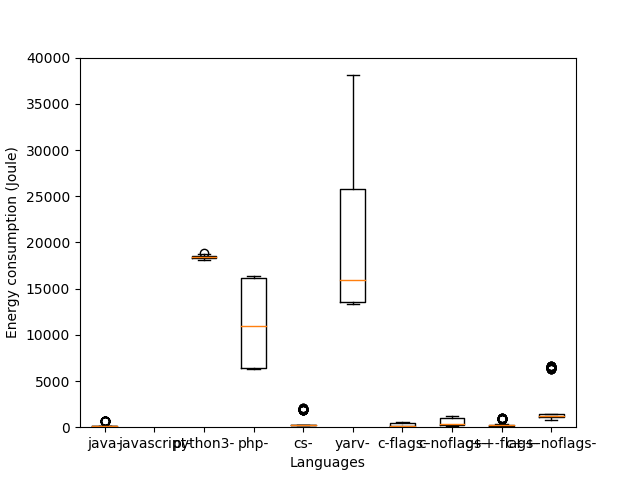
\includegraphics[width=.6\textwidth]{graphs/mandelbrot_BOXoverview3.png}
    \caption{The box plot of the different programs in a programming language for the problem Mandelbrot on \textit{node28}.}
    \label{fig:box-mandelbrot3}
\end{figure}

% Please add the following required packages to your document preamble:
% \usepackage{graphicx}
\begin{table}[h]
\centering
\resizebox{\textwidth}{!}{%
\begin{tabular}{|l|c|c|c|c|c|c|c|c|c|c|}
\hline
 & \multicolumn{1}{l|}{Java} & \multicolumn{1}{l|}{JavaScript} & \multicolumn{1}{l|}{Python} & \multicolumn{1}{l|}{PHP} & \multicolumn{1}{l|}{C\#} & \multicolumn{1}{l|}{Ruby} & \multicolumn{1}{l|}{C-flags} & \multicolumn{1}{l|}{C-noflags} & \multicolumn{1}{l|}{C++-flags} & \multicolumn{1}{l|}{C++-noflags} \\ \hline
Java & 0 & & + & + & + & + & - & + & - & +\\ \hline
JavaScript & & & & & & & & & & \\ \hline
Python& - & & 0 & - & - & Unknown & - & - & - & -\\ \hline
PHP & - & & + & 0 & - & + & - & - & - & -\\ \hline
C\# & - & & + & + & 0 & + & - & Unknown & - & +\\ \hline
Ruby & - & & Unknown & - & - & 0 & - & - & - & -\\ \hline
C-flags & + & & + & + & + & + & 0 & + & Unknown & +\\ \hline
C-noflags & - & & + & + & Unknown & + & - & 0 & - & +\\ \hline
C++-flags & + & & + & + & + & + & Unknown & + & 0 & +\\ \hline
C++-noflags & - & & + & + & - & + & - & - & - & 0\\ \hline
\end{tabular}%
}
\caption{The comparison of the different languages for the Mandelbrot problem on \textit{node28}. A \textit{+} means that the language on the row has a lower energy consumption then the language on the column, the opposite for \textit{-}, and the \textit{Unknown} means that we could not reject the null hypothesis.}
\label{tab:lang-mandelbrot3}
\end{table}

\begin{figure}[h]
    \centering
    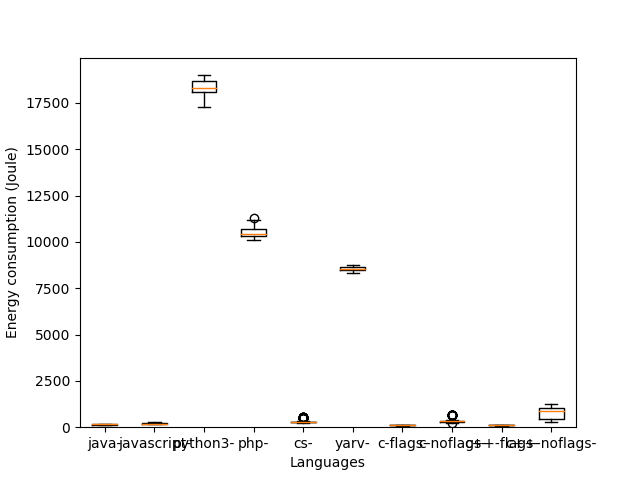
\includegraphics[width=.6\textwidth]{graphs/nbody_BOXoverview3.png}
    \caption{The box plot of the different programs in a programming language for the problem Nbody on \textit{node28}.}
    \label{fig:box-nbody3}
\end{figure}

% Please add the following required packages to your document preamble:
% \usepackage{graphicx}
\begin{table}[h]
\centering
\resizebox{\textwidth}{!}{%
\begin{tabular}{|l|c|c|c|c|c|c|c|c|c|c|}
\hline
 & \multicolumn{1}{l|}{Java} & \multicolumn{1}{l|}{JavaScript} & \multicolumn{1}{l|}{Python} & \multicolumn{1}{l|}{PHP} & \multicolumn{1}{l|}{C\#} & \multicolumn{1}{l|}{Ruby} & \multicolumn{1}{l|}{C-flags} & \multicolumn{1}{l|}{C-noflags} & \multicolumn{1}{l|}{C++-flags} & \multicolumn{1}{l|}{C++-noflags} \\ \hline
Java& 0 & + & + & + & + & + & - & + & - & +\\ \hline
JavaScript & - & 0 & + & + & + & + & - & + & - & +\\ \hline
Python& - & - & 0 & - & - & - & - & - & - & -\\ \hline
PHP & - & - & + & 0 & - & - & - & - & - & -\\ \hline
C\# & - & - & + & + & 0 & + & - & + & - & +\\ \hline
Ruby & - & - & + & + & - & 0 & - & - & - & -\\ \hline
C-flags & + & + & + & + & + & + & 0 & + & Unknown & +\\ \hline
C-noflags & - & - & + & + & - & + & - & 0 & - & +\\ \hline
C++-flags & + & + & + & + & + & + & Unknown & + & 0 & +\\ \hline
C++-noflags & - & - & + & + & - & + & - & - & - & 0\\ \hline
\end{tabular}%
}
\caption{The comparison of the different languages for the Nbody problem on \textit{node28}. A \textit{+} means that the language on the row has a lower energy consumption then the language on the column, the opposite for \textit{-}, and the \textit{Unknown} means that we could not reject the null hypothesis.}
\label{tab:lang-nbody3}
\end{table}

\begin{figure}[h]
    \centering
    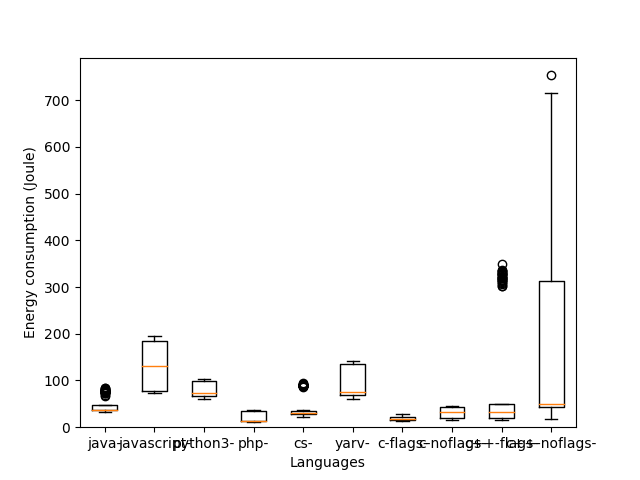
\includegraphics[width=.6\textwidth]{graphs/revcomp_BOXoverview3.png}
    \caption{The box plot of the different programs in a programming language for the problem Revcomp on \textit{node28}.}
    \label{fig:box-revcomp3}
\end{figure}

% Please add the following required packages to your document preamble:
% \usepackage{graphicx}
\begin{table}[h]
\centering
\resizebox{\textwidth}{!}{%
\begin{tabular}{|l|c|c|c|c|c|c|c|c|c|c|}
\hline
 & \multicolumn{1}{l|}{Java} & \multicolumn{1}{l|}{JavaScript} & \multicolumn{1}{l|}{Python} & \multicolumn{1}{l|}{PHP} & \multicolumn{1}{l|}{C\#} & \multicolumn{1}{l|}{Ruby} & \multicolumn{1}{l|}{C-flags} & \multicolumn{1}{l|}{C-noflags} & \multicolumn{1}{l|}{C++-flags} & \multicolumn{1}{l|}{C++-noflags} \\ \hline
Java& 0 & + & + & - & - & + & - & - & - & +\\ \hline
JavaScript& - & 0 & - & - & - & - & - & - & - & -\\ \hline
Python& - & + & 0 & - & - & + & - & - & - & -\\ \hline
PHP & + & + & + & 0 & + & + & + & + & + & +\\ \hline
C\# & + & + & + & - & 0 & + & - & Unknown & Unknown & +\\ \hline
Ruby& - & + & - & - & - & 0 & - & - & - & -\\ \hline
C-flags & + & + & + & - & + & + & 0 & + & + & +\\ \hline
C-noflags & + & + & + & - & Unknown & + & - & 0 & Unknown & +\\ \hline
C++-flags & + & + & + & - & Unknown & + & - & Unknown & 0 & +\\ \hline
C++-noflags & - & + & + & - & - & + & - & - & - & 0\\ \hline
\end{tabular}%
}
\caption{The comparison of the different languages for the Revcomp problem on \textit{node28}. A \textit{+} means that the language on the row has a lower energy consumption then the language on the column, the opposite for \textit{-}, and the \textit{Unknown} means that we could not reject the null hypothesis.}
\label{tab:lang-revcomp3}
\end{table}

\begin{figure}[h]
    \centering
    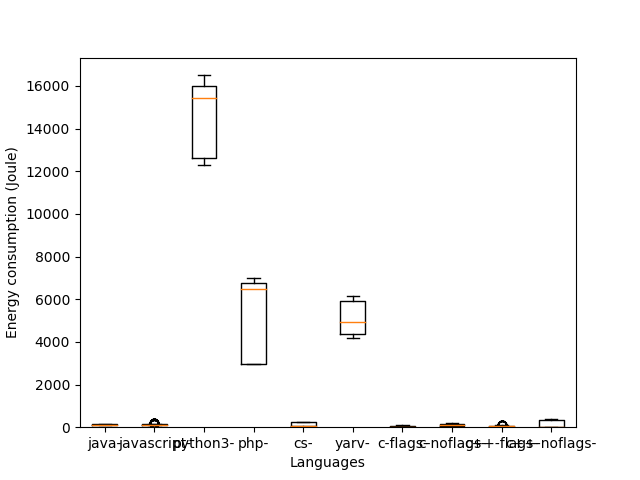
\includegraphics[width=.6\textwidth]{graphs/spectralnorm_BOXoverview3.png}
    \caption{The box plot of the different programs in a programming language for the problem Spectralnorm on \textit{node29}.}
    \label{fig:box-spectralnorm3}
\end{figure}

% Please add the following required packages to your document preamble:
% \usepackage{graphicx}
\begin{table}[h]
\centering
\resizebox{\textwidth}{!}{%
\begin{tabular}{|l|c|c|c|c|c|c|c|c|c|c|}
\hline
 & \multicolumn{1}{l|}{Java} & \multicolumn{1}{l|}{JavaScript} & \multicolumn{1}{l|}{Python} & \multicolumn{1}{l|}{PHP} & \multicolumn{1}{l|}{C\#} & \multicolumn{1}{l|}{Ruby} & \multicolumn{1}{l|}{C-flags} & \multicolumn{1}{l|}{C-noflags} & \multicolumn{1}{l|}{C++-flags} & \multicolumn{1}{l|}{C++-noflags} \\ \hline
Java& 0 & - & + & + & Unknown & + & - & - & - & -\\ \hline
JavaScript& + & 0 & + & + & Unknown & + & - & - & - & -\\ \hline
Python& - & - & 0 & - & - & - & - & - & - & -\\ \hline
PHP & - & - & + & 0 & - & Unknown & - & - & - & -\\ \hline
C\# & Unknown & Unknown & + & + & 0 & + & - & Unknown & - & Unknown\\ \hline
Ruby& - & - & + & Unknown & - & 0 & - & - & - & -\\ \hline
C-flags & + & + & + & + & + & + & 0 & + & + & +\\ \hline
C-noflags & + & + & + & + & Unknown & + & - & 0 & - & -\\ \hline
C++-flags & + & + & + & + & + & + & - & + & 0 & +\\ \hline
C++-noflags & + & + & + & + & Unknown & + & - & + & - & 0\\ \hline
\end{tabular}%
}
\caption{The comparison of the different languages for the Spectralnorm problem on \textit{node28}. A \textit{+} means that the language on the row has a lower energy consumption then the language on the column, the opposite for \textit{-}, and the \textit{Unknown} means that we could not reject the null hypothesis.}
\label{tab:lang-spectralnorm3}
\end{table}

\begin{table}[h]
\centering
\begin{tabular}{|l|l|l|l|}
\hline
Program 1 & Program 2 & p-less & p-greater \\ \hline
java-3.problem0 & java-6.problem0 & 0.266 & 0.740 \\ \hline
javascript-1.problem2 & javascript-2.problem2 & 0.829 & 0.176 \\ \hline
javascript-1.problem2 & javascript-3.problem2 & 0.413 & 0.594 \\ \hline
javascript-2.problem2 & javascript-3.problem2 & 0.197 & 0.808 \\ \hline
javascript-1.problem6 & javascript-3.problem6 & 0.532 & 0.475 \\ \hline
javascript-1.problem6 & javascript-5.problem6 & 0.272 & 0.734 \\ \hline
javascript-3.problem6 & javascript-5.problem6 & 0.243 & 0.763 \\ \hline
python3-2.problem3 & python3-5.problem3 & 0.488 & 0.520 \\ \hline
cs-3.problem3 & cs-4.problem3 & 0.088 & 0.915 \\ \hline
cs-3.problem4 & cs-5.problem4 & 0.622 & 0.385 \\ \hline
cs-4.problem4 & cs-6.problem4 & 0.493 & 0.515 \\ \hline
c-noflags-1.problem2 & c-noflags-2.problem2 & 0.882 & 0.122 \\ \hline
c-flags-2.problem4 & c-flags-3.problem4 & 0.230 & 0.776 \\ \hline
c-noflags-1.problem4 & c-noflags-6.problem4 & 0.218 & 0.787 \\ \hline
c-flags-3.problem5 & c-flags-6.problem5 & 0.175 & 0.830 \\ \hline
c-noflags-4.problem5 & c-noflags-5.problem5 & 0.090 & 0.912 \\ \hline
c++-flags-1.problem0 & c++-flags-8.problem0 & 0.571 & 0.436 \\ \hline
c++-noflags-1.problem0 & c++-noflags-3.problem0 & 0.883 & 0.121 \\ \hline
c++-noflags-1.problem0 & c++-noflags-8.problem0 & 0.874 & 0.130 \\ \hline
c++-noflags-3.problem0 & c++-noflags-8.problem0 & 0.453 & 0.555 \\ \hline
c++-flags-1.problem2 & c++-flags-2.problem2 & 0.317 & 0.690 \\ \hline
c++-flags-3.problem4 & c++-flags-8.problem4 & 0.168 & 0.837 \\ \hline
c++-flags-4.problem4 & c++-flags-6.problem4 & 0.225 & 0.781 \\ \hline
c++-noflags-5.problem6 & c++-noflags-6.problem6 & 0.374 & 0.633 \\ \hline
\end{tabular}
\caption{The programs result from \textit{node28} where the null hypothesis that they are from the same distribution could not be reject for the Mann Whitney U one-sided test less and bigger.}
\label{tab:programs_equal3}
\end{table}

%------------------------------------------------------------------
%------------------------------------------------------------------
%------------------------------------------------------------------
%------------------------------------------------------------------
%--------------------HERE TO NEXT CHAPTER--------------------------
%------------------------------------------------------------------
%------------------------------------------------------------------
%------------------------------------------------------------------
%------------------------------------------------------------------

\chapter{Node29}
\label{app:node29}
\begin{figure}[h]
    \centering
    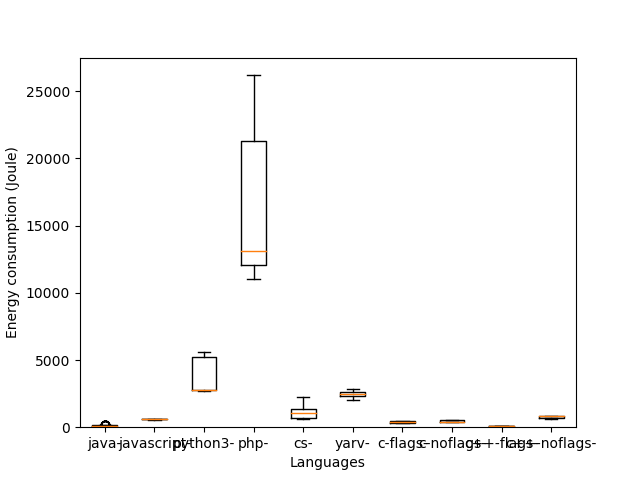
\includegraphics[width=.6\textwidth]{graphs/binarytrees_BOXoverview2.png}
    \caption{The box plot of the different programs in a programming language for the problem Binarytrees on \textit{node29}.}
    \label{fig:box-binarytrees2}
\end{figure}

\begin{table}[h]
\centering
\resizebox{\textwidth}{!}{%
\begin{tabular}{|l|c|c|c|c|c|c|c|c|c|c|}
\hline
 & \multicolumn{1}{l|}{Java} & \multicolumn{1}{l|}{JavaScript} & \multicolumn{1}{l|}{Python} & \multicolumn{1}{l|}{PHP} & \multicolumn{1}{l|}{C\#} & \multicolumn{1}{l|}{Ruby} & \multicolumn{1}{l|}{C-flags} & \multicolumn{1}{l|}{C-noflags} & \multicolumn{1}{l|}{C++-flags} & \multicolumn{1}{l|}{C++-noflags} \\ \hline
Java & 0 & + & + & + & + & + & + & + & - & +\\ \hline
JavaScript & - & 0 & + & + & + & + & - & - & - & +\\ \hline
Python & - & - & 0 & + & - & - & - & - & - & -\\ \hline
PHP & - & - & - & 0 & - & - & - & - & - & -\\ \hline
C\# & - & - & + & + & 0 & + & - & - & - & -\\ \hline
Ruby & - & - & + & + & - & 0 & - & - & - & -\\ \hline
C-flags & - & + & + & + & + & + & 0 & + & - & +\\ \hline
C-noflags & - & + & + & + & + & + & - & 0 & - & +\\ \hline
C++-flags & + & + & + & + & + & + & + & + & 0 & +\\ \hline
C++-noflags & - & - & + & + & + & + & - & - & - & 0\\ \hline
\end{tabular}%
}
\caption{The comparison of the different languages for the Binarytrees problem on \textit{node29}. A \textit{+} means that the language on the row has a lower energy consumption then the language on the column, the opposite for \textit{-}.}
\label{tab:lang-binarytrees2}
\end{table}

\begin{figure}[h]
    \centering
    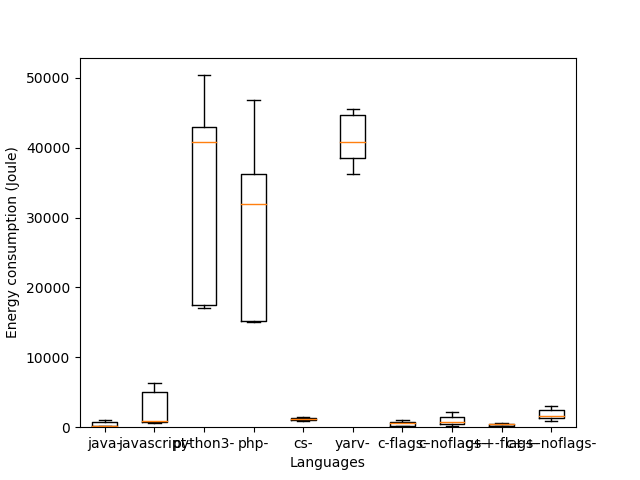
\includegraphics[width=.6\textwidth]{graphs/fannkuchredux_BOXoverview2.png}
    \caption{The box plot of the different programs in a programming language for the problem Fannkuchredux on \textit{node29}.}
    \label{fig:box-fannkuchredux2}
\end{figure}

\begin{table}[h]
\centering
\resizebox{\textwidth}{!}{%
\begin{tabular}{|l|c|c|c|c|c|c|c|c|c|c|}
\hline
 & \multicolumn{1}{l|}{Java} & \multicolumn{1}{l|}{JavaScript} & \multicolumn{1}{l|}{Python} & \multicolumn{1}{l|}{PHP} & \multicolumn{1}{l|}{C\#} & \multicolumn{1}{l|}{Ruby} & \multicolumn{1}{l|}{C-flags} & \multicolumn{1}{l|}{C-noflags} & \multicolumn{1}{l|}{C++-flags} & \multicolumn{1}{l|}{C++-noflags} \\ \hline
Java & 0 & + & + & + & + & + & + & + & Unknown & + \\ \hline
JavaScript & - & 0 & + & + & + & + & - & - & - & + \\ \hline
Python & - & - & 0 & - & - & Unknown & - & - & - & - \\ \hline
PHP & - & - & + & 0 & - & + & - & - & - & - \\ \hline
C\# & - & - & + & + & 0 & + & - & - & - & +\\ \hline
Ruby & - & - & Unknown & - & - & 0 & - & - & - & -\\ \hline
C-flags & - & + & + & + & + & + & 0 & + & - & +\\ \hline
C-noflags & - & + & + & + & + & + & - & 0 & - & +\\ \hline
C++-flags & Unknown & + & + & + & + & + & + & + & 0 & +\\ \hline
C++-noflags & - & - & + & + & - & + & - & - & - & 0\\ \hline
\end{tabular}%
}
\caption{The comparison of the different languages for the Fannkuchredux problem on \textit{node29}. A \textit{+} means that the language on the row has a lower energy consumption then the language on the column, the opposite for \textit{-}.}
\label{tab:lang-fannkuchredux2}
\end{table}

\begin{figure}[h]
    \centering
    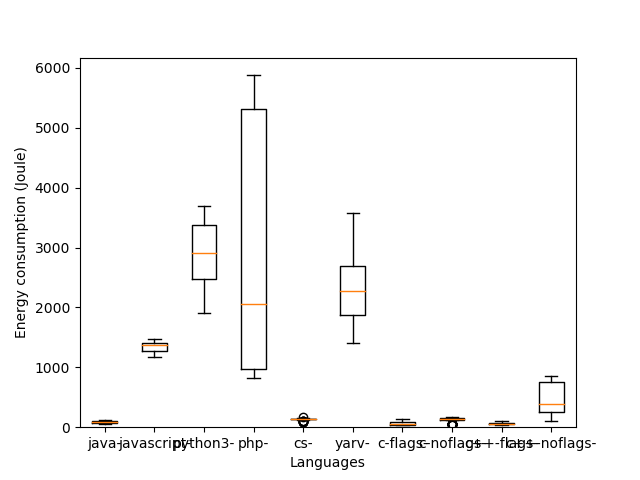
\includegraphics[width=.6\textwidth]{graphs/fasta_BOXoverview2.png}
    \caption{The box plot of the different programs in a programming language for the problem Fasta on \textit{node29}.}
    \label{fig:box-fasta2}
\end{figure}

% Please add the following required packages to your document preamble:
% \usepackage{graphicx}
\begin{table}[h]
\centering
\resizebox{\textwidth}{!}{%
\begin{tabular}{|l|c|c|c|c|c|c|c|c|c|c|}
\hline
 & \multicolumn{1}{l|}{Java} & \multicolumn{1}{l|}{JavaScript} & \multicolumn{1}{l|}{Python} & \multicolumn{1}{l|}{PHP} & \multicolumn{1}{l|}{C\#} & \multicolumn{1}{l|}{Ruby} & \multicolumn{1}{l|}{C-flags} & \multicolumn{1}{l|}{C-noflags} & \multicolumn{1}{l|}{C++-flags} & \multicolumn{1}{l|}{C++-noflags} \\ \hline
Java & 0 & + & + & + & + & + & - & + & - & + \\ \hline
JavaScript & - & 0 & + & + & - & + & - & - & - & - \\ \hline
Python & - & - & 0 & - & - & - & - & - & - & - \\ \hline
PHP & - & - & + & 0 & - & Unknown & - & - & - & - \\ \hline
C\# & - & + & + & + & 0 & + & - & Unknown & - & + \\ \hline
Ruby & - & - & + & Unknown & - & 0 & - & - & - & - \\ \hline
C-flags & + & + & + & + & + & + & 0 & + & Unknown & + \\ \hline
C-noflags & - & + & + & + & Unknown & + & - & 0 & - & + \\ \hline
C++-flags & + & + & + & + & + & + & Unknown & + & 0 & + \\ \hline
C++-noflags & - & + & + & + & - & + & - & - & - & 0 \\ \hline
\end{tabular}%
}
\caption{The comparison of the different languages for the Fasta problem on \textit{node29}. A \textit{+} means that the language on the row has a lower energy consumption then the language on the column, the opposite for \textit{-}, and the \textit{Unknown} means that we could not reject the null hypothesis.}
\label{tab:lang-fasta2}
\end{table}

\begin{figure}[h]
    \centering
    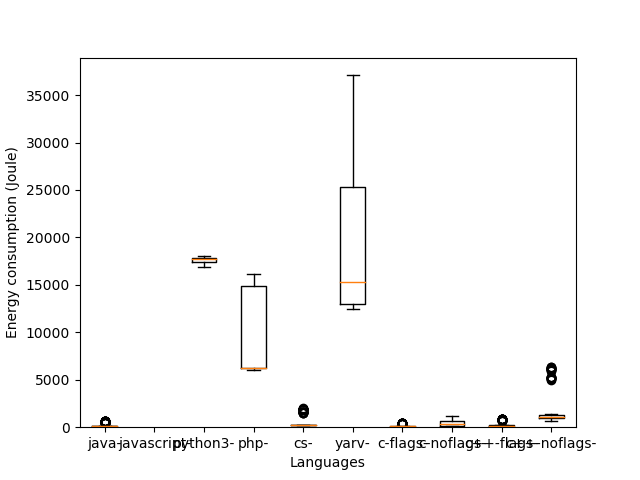
\includegraphics[width=.6\textwidth]{graphs/mandelbrot_BOXoverview2.png}
    \caption{The box plot of the different programs in a programming language for the problem Mandelbrot on \textit{node29}.}
    \label{fig:box-mandelbrot2}
\end{figure}

% Please add the following required packages to your document preamble:
% \usepackage{graphicx}
\begin{table}[h]
\centering
\resizebox{\textwidth}{!}{%
\begin{tabular}{|l|c|c|c|c|c|c|c|c|c|c|}
\hline
 & \multicolumn{1}{l|}{Java} & \multicolumn{1}{l|}{JavaScript} & \multicolumn{1}{l|}{Python} & \multicolumn{1}{l|}{PHP} & \multicolumn{1}{l|}{C\#} & \multicolumn{1}{l|}{Ruby} & \multicolumn{1}{l|}{C-flags} & \multicolumn{1}{l|}{C-noflags} & \multicolumn{1}{l|}{C++-flags} & \multicolumn{1}{l|}{C++-noflags} \\ \hline
Java & 0 & & + & + & + & + & - & + & - & +\\ \hline
JavaScript & & & & & & & & & & \\ \hline
Python& - & & 0 & - & - & - & - & - & - & -\\ \hline
PHP & - & & + & 0 & - & + & - & - & - & -\\ \hline
C\# & - & & + & + & 0 & + & - & Unknown & - & +\\ \hline
Ruby & - & & + & - & - & 0 & - & - & - & -\\ \hline
C-flags & + & & + & + & + & + & 0 & + & Unknown & +\\ \hline
C-noflags & - & & + & + & Unknown & + & - & 0 & - & +\\ \hline
C++-flags & + & & + & + & + & + & Unknown & + & 0 & +\\ \hline
C++-noflags & - & & + & + & - & + & - & - & - & 0\\ \hline
\end{tabular}%
}
\caption{The comparison of the different languages for the Mandelbrot problem on \textit{node29}. A \textit{+} means that the language on the row has a lower energy consumption then the language on the column, the opposite for \textit{-}, and the \textit{Unknown} means that we could not reject the null hypothesis.}
\label{tab:lang-mandelbrot2}
\end{table}

\begin{figure}[h]
    \centering
    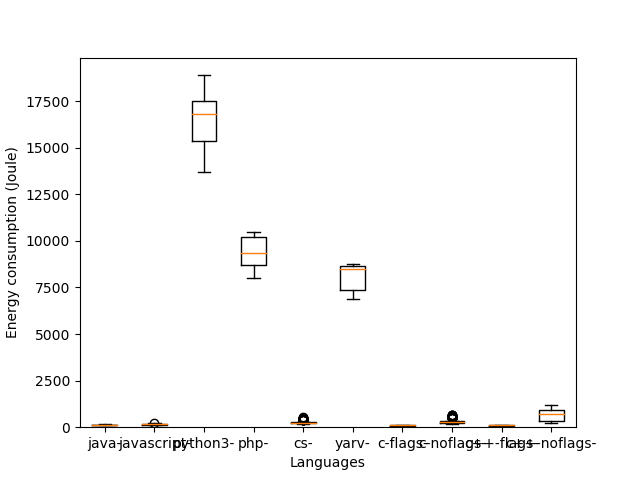
\includegraphics[width=.6\textwidth]{graphs/nbody_BOXoverview2.png}
    \caption{The box plot of the different programs in a programming language for the problem Nbody on \textit{node29}.}
    \label{fig:box-nbody2}
\end{figure}

% Please add the following required packages to your document preamble:
% \usepackage{graphicx}
\begin{table}[h]
\centering
\resizebox{\textwidth}{!}{%
\begin{tabular}{|l|c|c|c|c|c|c|c|c|c|c|}
\hline
 & \multicolumn{1}{l|}{Java} & \multicolumn{1}{l|}{JavaScript} & \multicolumn{1}{l|}{Python} & \multicolumn{1}{l|}{PHP} & \multicolumn{1}{l|}{C\#} & \multicolumn{1}{l|}{Ruby} & \multicolumn{1}{l|}{C-flags} & \multicolumn{1}{l|}{C-noflags} & \multicolumn{1}{l|}{C++-flags} & \multicolumn{1}{l|}{C++-noflags} \\ \hline
Java& 0 & + & + & + & + & + & - & + & - & +\\ \hline
JavaScript & - & 0 & + & + & + & + & - & + & - & +\\ \hline
Python& - & - & 0 & - & - & - & - & - & - & -\\ \hline
PHP & - & - & + & 0 & - & - & - & - & - & -\\ \hline
C\# & - & - & + & + & 0 & + & - & + & - & +\\ \hline
Ruby & - & - & + & + & - & 0 & - & - & - & -\\ \hline
C-flags & + & + & + & + & + & + & 0 & + & Unknown & +\\ \hline
C-noflags & - & - & + & + & - & + & - & 0 & - & +\\ \hline
C++-flags & + & + & + & + & + & + & Unknown & + & 0 & +\\ \hline
C++-noflags & - & - & + & + & - & + & - & - & - & 0\\ \hline
\end{tabular}%
}
\caption{The comparison of the different languages for the Nbody problem on \textit{node29}. A \textit{+} means that the language on the row has a lower energy consumption then the language on the column, the opposite for \textit{-}, and the \textit{Unknown} means that we could not reject the null hypothesis.}
\label{tab:lang-nbody2}
\end{table}

\begin{figure}[h]
    \centering
    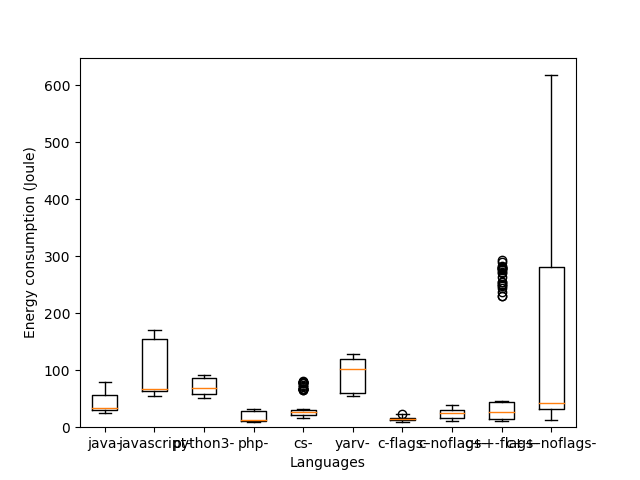
\includegraphics[width=.6\textwidth]{graphs/revcomp_BOXoverview2.png}
    \caption{The box plot of the different programs in a programming language for the problem Revcomp on \textit{node29}.}
    \label{fig:box-revcomp2}
\end{figure}

% Please add the following required packages to your document preamble:
% \usepackage{graphicx}
\begin{table}[h]
\centering
\resizebox{\textwidth}{!}{%
\begin{tabular}{|l|c|c|c|c|c|c|c|c|c|c|}
\hline
 & \multicolumn{1}{l|}{Java} & \multicolumn{1}{l|}{JavaScript} & \multicolumn{1}{l|}{Python} & \multicolumn{1}{l|}{PHP} & \multicolumn{1}{l|}{C\#} & \multicolumn{1}{l|}{Ruby} & \multicolumn{1}{l|}{C-flags} & \multicolumn{1}{l|}{C-noflags} & \multicolumn{1}{l|}{C++-flags} & \multicolumn{1}{l|}{C++-noflags} \\ \hline
Java& 0 & + & + & - & - & + & - & - & - & +\\ \hline
JavaScript& - & 0 & - & - & - & - & - & - & - & -\\ \hline
Python& - & + & 0 & - & - & + & - & - & - & -\\ \hline
PHP & + & + & + & 0 & + & + & Unknown & + & + & +\\ \hline
C\# & + & + & + & - & 0 & + & - & - & Unknown & +\\ \hline
Ruby& - & + & - & - & - & 0 & - & - & - & -\\ \hline
C-flags & + & + & + & Unknown & + & + & 0 & + & + & +\\ \hline
C-noflags & + & + & + & - & + & + & - & 0 & + & +\\ \hline
C++-flags & + & + & + & - & Unknown & + & - & - & 0 & +\\ \hline
C++-noflags & - & + & + & - & - & + & - & - & - & 0\\ \hline
\end{tabular}%
}
\caption{The comparison of the different languages for the Revcomp problem on \textit{node29}. A \textit{+} means that the language on the row has a lower energy consumption then the language on the column, the opposite for \textit{-}, and the \textit{Unknown} means that we could not reject the null hypothesis.}
\label{tab:lang-revcomp2}
\end{table}

\begin{figure}[h]
    \centering
    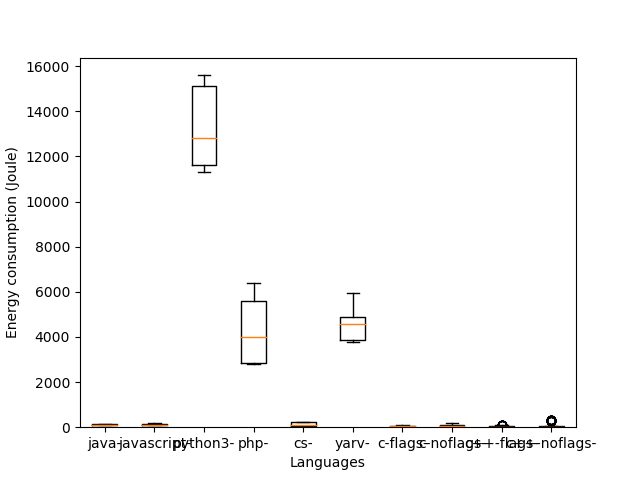
\includegraphics[width=.6\textwidth]{graphs/spectralnorm_BOXoverview2.png}
    \caption{The box plot of the different programs in a programming language for the problem Spectralnorm on \textit{node29}.}
    \label{fig:box-spectralnorm2}
\end{figure}

% Please add the following required packages to your document preamble:
% \usepackage{graphicx}
\begin{table}[h]
\centering
\resizebox{\textwidth}{!}{%
\begin{tabular}{|l|c|c|c|c|c|c|c|c|c|c|}
\hline
 & \multicolumn{1}{l|}{Java} & \multicolumn{1}{l|}{JavaScript} & \multicolumn{1}{l|}{Python} & \multicolumn{1}{l|}{PHP} & \multicolumn{1}{l|}{C\#} & \multicolumn{1}{l|}{Ruby} & \multicolumn{1}{l|}{C-flags} & \multicolumn{1}{l|}{C-noflags} & \multicolumn{1}{l|}{C++-flags} & \multicolumn{1}{l|}{C++-noflags} \\ \hline
Java& 0 & - & + & + & Unknown & + & - & - & - & -\\ \hline
JavaScript& + & 0 & + & + & Unknown & + & - & - & - & -\\ \hline
Python& - & - & 0 & - & - & - & - & - & - & -\\ \hline
PHP & - & - & + & 0 & - & Unknown & - & - & - & -\\ \hline
C\# & Unknown & Unknown & + & + & 0 & + & - & Unknown & - & Unknown\\ \hline
Ruby& - & - & + & Unknown & - & 0 & - & - & - & -\\ \hline
C-flags & + & + & + & + & + & + & 0 & + & + & +\\ \hline
C-noflags & + & + & + & + & Unknown & + & - & 0 & - & -\\ \hline
C++-flags & + & + & + & + & + & + & - & + & 0 & +\\ \hline
C++-noflags & + & + & + & + & Unknown & + & - & + & - & 0\\ \hline
\end{tabular}%
}
\caption{The comparison of the different languages for the Spectralnorm problem on \textit{node29}. A \textit{+} means that the language on the row has a lower energy consumption then the language on the column, the opposite for \textit{-}, and the \textit{Unknown} means that we could not reject the null hypothesis.}
\label{tab:lang-spectralnorm2}
\end{table}

\begin{table}[h]
\centering
\small
\begin{adjustbox}{height=0.5\textheight}
\begin{tabular}{|l|l|l|l|l|}
\hline
Program 1 & Program 2 & p-less & p-greater & K-S test\\ \hline
java-2.problem0 & java-3.problem0 & 0.937 & 0.066 & Unknown\\ \hline
java-2.problem0 & java-6.problem0 & 0.820 & 0.186 & Unknown\\ \hline
java-3.problem0 & java-6.problem0 & 0.164 & 0.842 & Unknown\\ \hline
java-2.problem3 & java-4.problem3 & 0.514 & 0.495 & Unknown\\ \hline
java-2.problem4 & java-3.problem4 & 0.864 & 0.142 & Unknown\\ \hline
java-4.problem5 & java-5.problem5 & 0.732 & 0.276 & Unknown\\ \hline
java-5.problem5 & java-6.problem5 & 0.915 & 0.089 & Unknown\\ \hline
javascript-1.problem2 & javascript-2.problem2 & 0.174 & 0.832 & Unknown \\ \hline
javascript-1.problem2 & javascript-3.problem2 & 0.106 & 0.898 & Unknown\\ \hline
javascript-2.problem2 & javascript-3.problem2 & 0.305 & 0.704 & Unknown\\ \hline
javascript-3.problem2 & javascript-4.problem2 & 0.120 & 0.884 & Unknown\\ \hline
javascript-1.problem4 & javascript-4.problem4 & 0.060 & 0.943 & Unknown\\ \hline
javascript-1.problem4 & javascript-5.problem4 & 0.053 & 0.950 & Unknown\\ \hline
javascript-4.problem4 & javascript-5.problem4 & 0.401 & 0.609 & Unknown\\ \hline
javascript-1.problem6 & javascript-3.problem6 & 0.658 & 0.352 & Unknown\\ \hline
javascript-1.problem6 & javascript-5.problem6 & 0.628 & 0.382 & Unknown\\ \hline
javascript-3.problem6 & javascript-5.problem6 & 0.495 & 0.516 & Unknown\\ \hline
cs-1.problem1 & cs-3.problem1 & 0.609 & 0.400 & Rejected\\ \hline
cs-1.problem1 & cs-4.problem1 & 0.606 & 0.404 & Rejected\\ \hline
cs-2.problem1 & cs-5.problem1 & 0.793 & 0.214 & Rejected\\ \hline
cs-2.problem1 & cs-6.problem1 & 0.909 & 0.095 & Rejected\\ \hline
cs-1.problem3 & cs-4.problem3 & 0.756 & 0.252 & Unknown\\ \hline
cs-3.problem3 & cs-4.problem3 & 0.372 & 0.638 & Unknown\\ \hline
cs-3.problem3 & cs-6.problem3 & 0.877 & 0.128 & Rejected\\ \hline
cs-4.problem3 & cs-6.problem3 & 0.855 & 0.151 & Unknown\\ \hline
cs-2.problem4 & cs-3.problem4 & 0.952 & 0.050 & Unknown\\ \hline
cs-3.problem4 & cs-5.problem4 & 0.882 & 0.123 & Unknown\\ \hline
cs-4.problem4 & cs-6.problem4 & 0.430 & 0.580 & Unknown\\ \hline
cs-4.problem4 & cs-8.problem4 & 0.945 & 0.058 & Unknown\\ \hline
cs-6.problem4 & cs-8.problem4 & 0.952 &0.050 & Unknown\\ \hline
cs-1.problem5 & cs-5.problem5 & 0.907 & 0.097 & Unknown\\ \hline
cs-2.problem5 & cs-5.problem5 & 0.157 & 0.849 & Unknown\\ \hline
yarv-1.problem1 & yarv-2.problem1 & 0.825 & 0.190 & Unknown\\ \hline
c-flags-2.problem2 & c-flags-5.problem2 & 0.292 & 0.716 & Rejected\\ \hline
c-noflags-1.problem2 & c-noflags-2.problem2 & 0.525 & 0.485 & Unknown\\ \hline
c-noflags-1.problem2 & c-noflags-5.problem2 & 0.200 & 0.806 & Unknown\\ \hline
c-noflags-1.problem2 & c-noflags-7.problem2 & 0.582 & 0.427 & Unknown\\ \hline
c-noflags-2.problem2 & c-noflags-5.problem2 & 0.224 & 0.783 & Unknown\\ \hline
c-noflags-2.problem2 & c-noflags-7.problem2 & 0.690 & 0.319 & Unknown\\ \hline
c-noflags-5.problem2 & c-noflags-7.problem2 & 0.861 & 0.145 & Unknown\\ \hline
c-flags-2.problem4 & c-flags-3.problem4 & 0.657 & 0.352 & Unknown\\ \hline
c-flags-2.problem4 & c-flags-6.problem4 & 0.470 & 0.540 & Unknown\\ \hline
c-flags-3.problem4 & c-flags-6.problem4 & 0.311 & 0.698 & Unknown\\ \hline
c-noflags-1.problem4 & c-noflags-6.problem4 & 0.410 & 0.599 & Unknown\\ \hline
c-flags-3.problem5 & c-flags-6.problem5 & 0.278 & 0.730 & Unknown\\ \hline
c-noflags-4.problem5 & c-noflags-5.problem5 & 0.300 & 0.708 & Unknown\\ \hline
c-noflags-4.problem6 & c-noflags-5.problem6 & 0.401 & 0.609 & Rejected\\ \hline
c++-noflags-1.problem0 & c++-noflags-3.problem0 & 0.340 & 0.669 & Unknown\\ \hline
c++-noflags-1.problem0 & c++-noflags-8.problem0 & 0.212 & 0.795 & Unknown\\ \hline
c++-noflags-3.problem0 & c++-noflags-8.problem0 & 0.398 & 0.612 & Unknown\\ \hline
c++-flags-4.problem1 & c++-flags-6.problem1 & 0.244 & 0.763 & Rejected\\ \hline
c++-flags-1.problem2 & c++-flags-2.problem2 & 0.676 & 0.333 & Unknown\\ \hline
c++-flags-1.problem2 & c++-flags-6.problem2 & 0.903 & 0.102 & Rejected\\ \hline
c++-flags-2.problem3 & c++-flags-5.problem3 & 0.790 & 0.217 & Unknown\\ \hline
c++-noflags-8.problem3 & c++-noflags-9.problem3 & 0.272 & 0.736 & Unknown\\ \hline
c++-flags-3.problem4 & c++-flags-8.problem4 & 0.642 & 0.367 & Unknown\\ \hline
c++-flags-4.problem4 & c++-flags-6.problem4 & 0.473 & 0.538 & Unknown\\ \hline
c++-noflags-1.problem4 & c++-noflags-6.problem4 & 0.277 & 0.731 & Unknown\\ \hline
c++-noflags-7.problem4 & c++-noflags-8.problem4 & 0.910 & 0.094 & Unknown\\ \hline
\end{tabular}
\end{adjustbox}
\caption{The programs result from \textit{node29} where the null hypothesis that they are from the same distribution could not be reject for the Mann Whitney U one-sided test less and bigger.}
\label{tab:programs_equal2}
\end{table}

%------------------------------------------------------------------
%------------------------------------------------------------------
%------------------------------------------------------------------
%------------------------------------------------------------------
%--------------------HERE TO NEXT CHAPTER--------------------------
%------------------------------------------------------------------
%------------------------------------------------------------------
%------------------------------------------------------------------
%------------------------------------------------------------------

\chapter{Correlation}
\label{app:corr}

\begin{figure}[h]
    \centering
    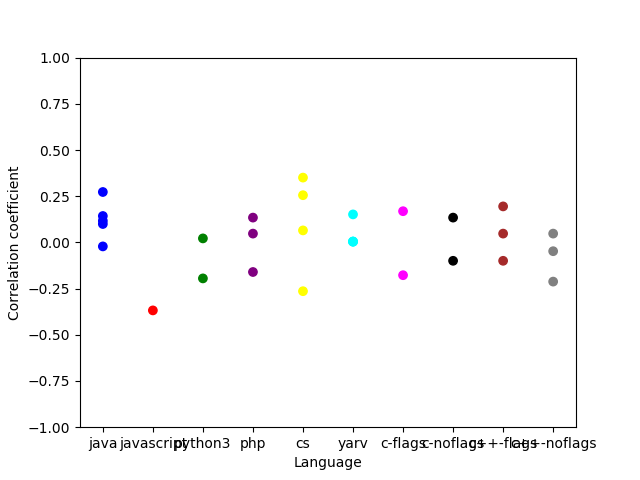
\includegraphics[width=.6\textwidth]{graphs/kendall_Binarytrees.png}
    \caption{The Kendall correlation score for every single program that solves the Binarytrees problem.}
    \label{fig:corr-binarytrees}
\end{figure}

\begin{figure}[h]
    \centering
    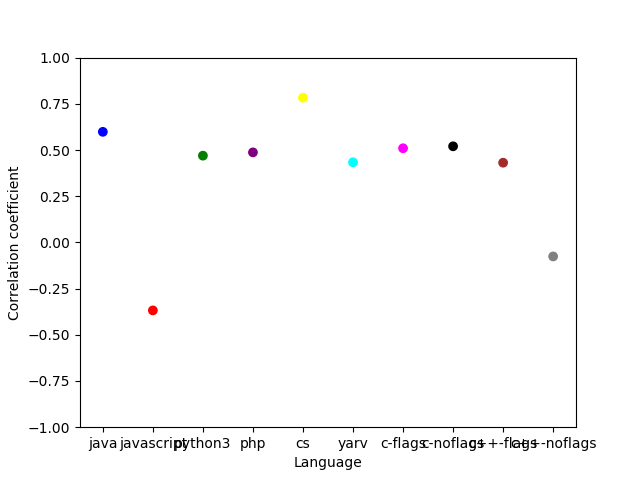
\includegraphics[width=.6\textwidth]{graphs/kendall-lang_Binarytrees.png}
    \caption{The Kendall correlation score for every programming language that solves the Binarytrees problem.}
    \label{fig:corr-lang-binarytrees}
\end{figure}

\begin{figure}[h]
    \centering
    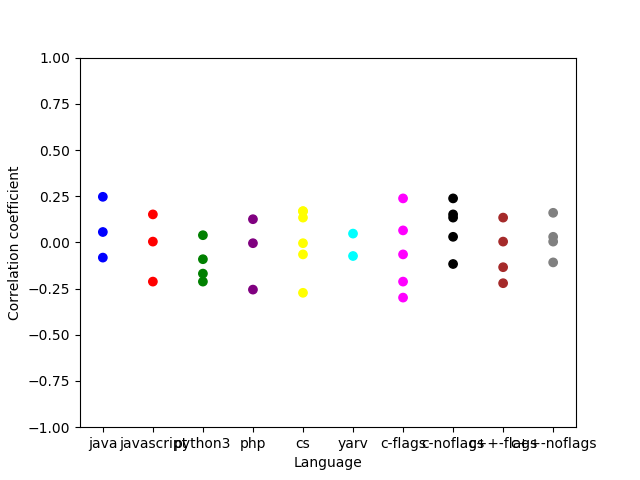
\includegraphics[width=.6\textwidth]{graphs/kendall_Fannkuchredux.png}
    \caption{The Kendall correlation score for every single program that solves the Fannkuchredux problem.}
    \label{fig:corr-fannkuchredux}
\end{figure}

\begin{figure}[h]
    \centering
    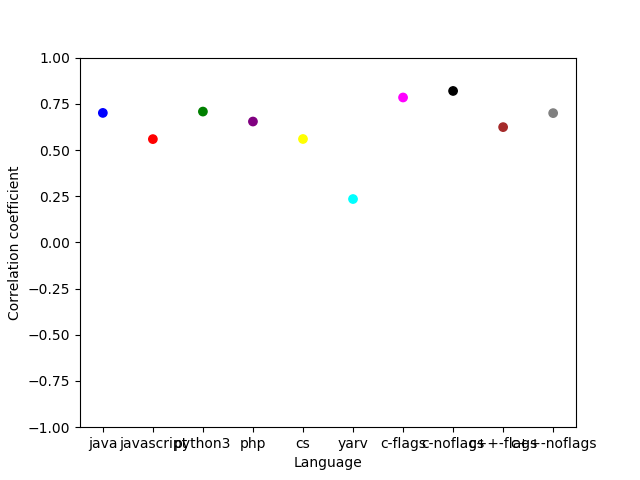
\includegraphics[width=.6\textwidth]{graphs/kendall-lang_Fannkuchredux.png}
    \caption{The Kendall correlation score for every programming language that solves the Fannkuchredux problem.}
    \label{fig:corr-lang-fannkuchredux}
\end{figure}

\begin{figure}[h]
    \centering
    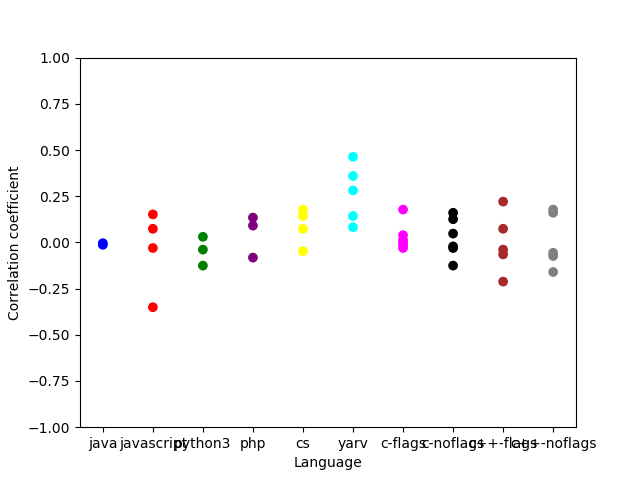
\includegraphics[width=.6\textwidth]{graphs/kendall_Fasta.png}
    \caption{The Kendall correlation score for every single program that solves the Fasta problem.}
    \label{fig:corr-fasta}
\end{figure}

\begin{figure}[h]
    \centering
    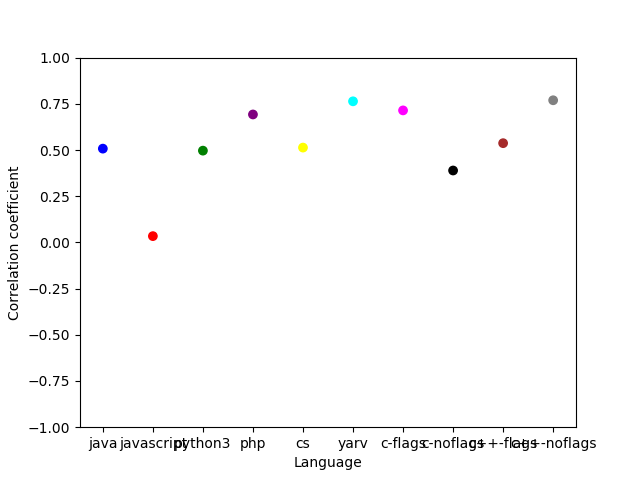
\includegraphics[width=.6\textwidth]{graphs/kendall-lang_Fasta.png}
    \caption{The Kendall correlation score for every programming language that solves the Fasta problem.}
    \label{fig:corr-lang-fasta}
\end{figure}

\begin{figure}[h]
    \centering
    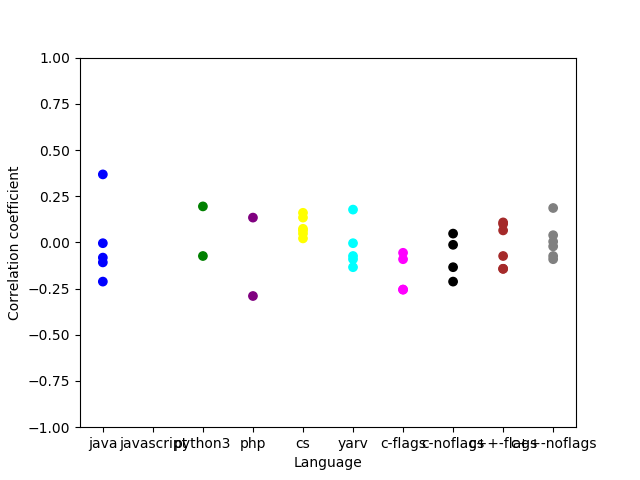
\includegraphics[width=.6\textwidth]{graphs/kendall_Mandelbrot.png}
    \caption{The Kendall correlation score for every single program that solves the Mandelbrot problem.}
    \label{fig:corr-mandelbrot}
\end{figure}

\begin{figure}[h]
    \centering
    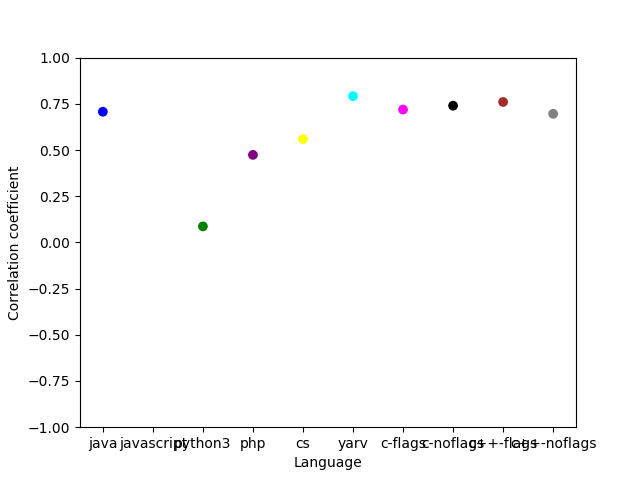
\includegraphics[width=.6\textwidth]{graphs/kendall-lang_Mandelbrot.png}
    \caption{The Kendall correlation score for every programming language that solves the Mandelbrot problem.}
    \label{fig:corr-lang-mandelbrot}
\end{figure}

\begin{figure}[h]
    \centering
    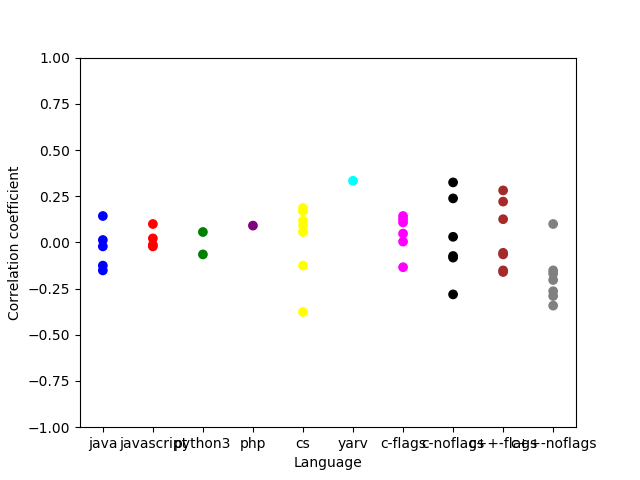
\includegraphics[width=.6\textwidth]{graphs/kendall_Nbody.png}
    \caption{The Kendall correlation score for every single program that solves the Nbody problem.}
    \label{fig:corr-nbody}
\end{figure}

\begin{figure}[h]
    \centering
    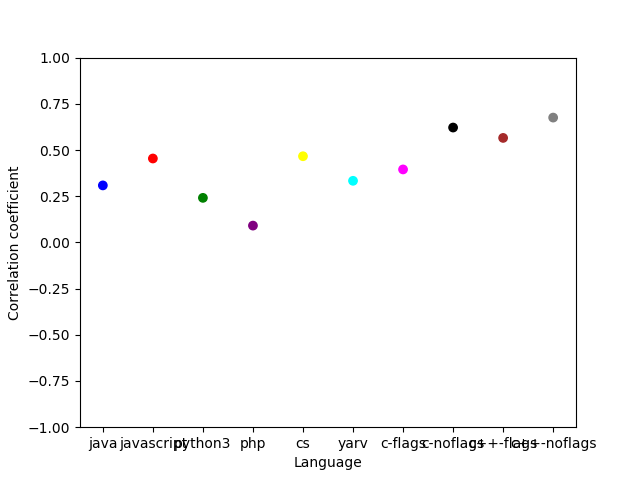
\includegraphics[width=.6\textwidth]{graphs/kendall-lang_Nbody.png}
    \caption{The Kendall correlation score for every programming language that solves the Nbody problem.}
    \label{fig:corr-lang-nbody}
\end{figure}

\begin{figure}[h]
    \centering
    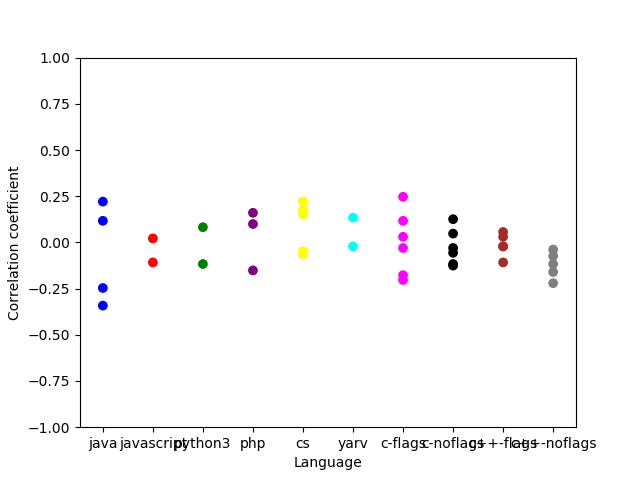
\includegraphics[width=.6\textwidth]{graphs/kendall_Revcomp.png}
    \caption{The Kendall correlation score for every single program that solves the Revcomp problem.}
    \label{fig:corr-revcomp}
\end{figure}

\begin{figure}[h]
    \centering
    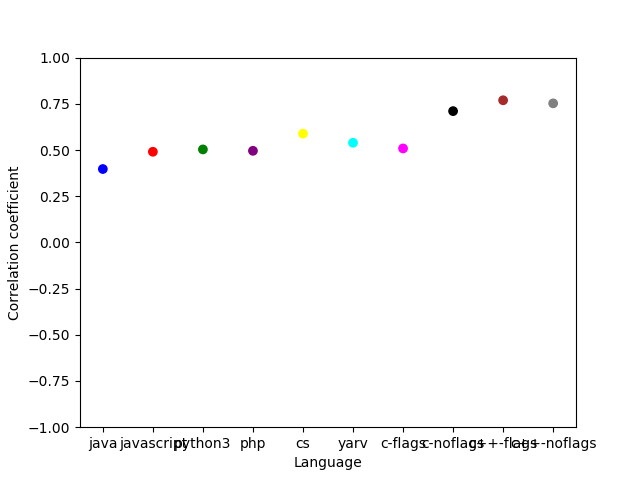
\includegraphics[width=.6\textwidth]{graphs/kendall-lang_Revcomp.png}
    \caption{The Kendall correlation score for every programming language that solves the Revcomp problem.}
    \label{fig:corr-lang-revcomp}
\end{figure}

\begin{figure}[h]
    \centering
    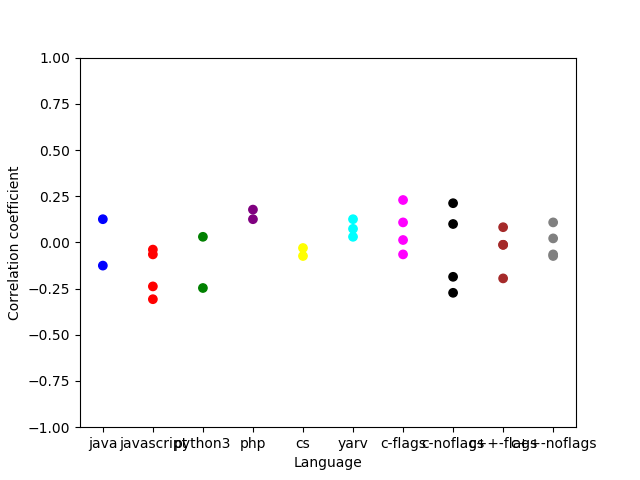
\includegraphics[width=.6\textwidth]{graphs/kendall_Spectralnorm.png}
    \caption{The Kendall correlation score for every single program that solves the Spectralnorm problem.}
    \label{fig:corr-spectralnorm}
\end{figure}

\begin{figure}[h]
    \centering
    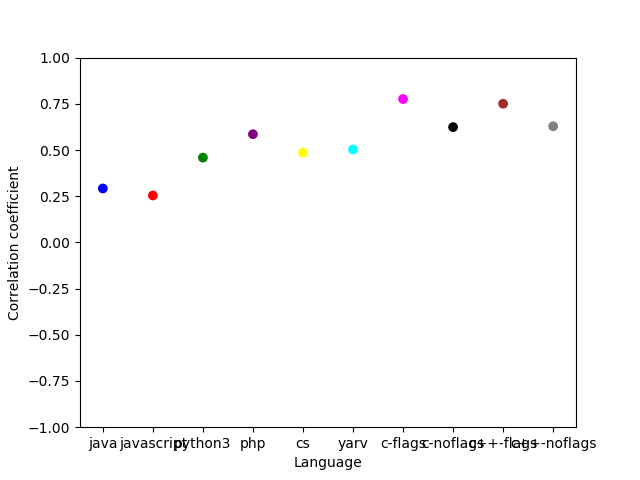
\includegraphics[width=.6\textwidth]{graphs/kendall-lang_Spectralnorm.png}
    \caption{The Kendall correlation score for every programming language that solves the Spectralnorm problem.}
    \label{fig:corr-lang-spectralnorm}
\end{figure}

\end{appendices}

%comment out in the final version
%\listoftodos[Notes]

\end{document}
